\documentclass[12pt,twoside]{article}
\usepackage{jmlda}
\usepackage{amsmath}
\usepackage{capt-of}
\usepackage{subcaption}
\usepackage{caption}
\newtheorem{theorem}{Theorem}
\newtheorem{lemma}[theorem]{Lemma}
\newtheorem{definition}{Definition}
\setcounter{secnumdepth}{3}
%\NOREVIEWERNOTES
\title{Анализ свойств моделей в задачах обучения с экспертом}
\author{А.\,И.~Базарова$^1$, А.\,В.~Грабовой$^1$, В.\,В.~Стрижов$^1$} % основной список авторов, выводимый в оглавление
\email{bazarova.ai@phystech.edu, grabovoy.av@phystech.edu, strijov@phystech.edu}
\organization{$^1$Московский физико-технический институт}
\abstract
    {В данной работе решается задача поиска заданного набора фигур на изображении в предположении, что фигуры являются кривыми второго порядка. Построение моделей машинного обучения основывается на информации о виде этих кривых и множестве их возможных преобразований. Такую информацию называют \textit{экспертными знаниями}, а метод машинного обучения, основанный на \textit{экспертных знаниях}, называют \textit{обучением с экспертом}.
    В работе предлагается отобразить кривые второго порядка в новое признаковое пространство, в котором каждая локальная модель является линейной моделью. Таким образом, распознавание кривых высших порядков может быть осуществлено при помощи композиции линейных моделей. В работе поставлена и решена задача оптимизации для поиска оптимальных параметров мультимодели.
    Качество работы предложенного метода сравнивается на синтетических данных и датасетах с реальными изображениями, которые включают в себя кривые второго порядка.

\bigskip
\textbf{Ключевые слова}: \emph {смесь моделей, обучение с экспертом, линейные модели}.
}
\begin{document}
\maketitle
\linenumbers
\section{Введение}
В работе предлагается метод \textit{обучения с экспертом}. 
Предметные знания экспертов используются в этом исследовании для повышения качества моделей машинного обучения.
Данные предметные знания назовем \textit{экспертными знаниями}. В данной работе в качестве  \texit{экспертных знаний} рассматриается информация о виде распознаваемой кривой и множестве ее допустимых преобразований. Метод машинного обучения, который учитывает \textit{экспертные знания} при построении моделей, назовем \textit{обучением с экспертом}. 

Работа сконцентрирована на распознавании изображений кривых второго и третьего порядка: квадрик, коник, кубик и поверхностей второго порядка. Данные фигуры выбраны для анализа, так как они являются простыми для аппроксимации линейными моделями фигурами. При этом эти фигуры требуется восстановить в прикладных задачах, таких как задача распознавания радужки глаза, задача описания трека частицы в Большом адронном коллайдере. Коэффициенты уравнений, описывающих данные кривые, аналитически выражаются через оптимальные параметры построенных в работе моделей.

Для каждого класса перечисленных кривых предлагается согласно экспертным данным отобразить точки на изображении в новое признаковое пространство и затем оптимально аппроксимировать кривую. Отображение строится таким образом, чтобы в новом признаковом описании каждая кривая описывалась линейной моделью. В данной работе рассматривается задача поиска фигур на изображении в предположении, что число и тип фигур на изображении заданы, а также заданы дополнительные преобразования фигур и их взаимное расположение. Для каждого типа фигур требуется построить признаковое описание, в котором фигура задается линейно. 

При распознавании нескольких кривых на одном изображении строится мультимодель, называемая смесью экспертов. Смесь экспертов~---~это мультимодель, которая линейно взвешивает локальные модели, аппроксимирующие выборку. Значения весовых коэффициентов зависят от того объекта, для которого производится предсказание. 

Примерами мультимоделей являются беггинг, градиентный бустинг и случайный лес решающих деревьев. Подход к мультимоделированию предполагает, что вклад каждого эксперта в ответ зависит от рассматриваемого объекта. Для восстановления этой зависимости смесь экспертов использует шлюзовую функцию. Она определяет значимость предсказания каждого эксперта~---~отдельной модели, входящей в смесь. Таким образом, ансамбль моделей включает два типа параметров: параметры локальных моделей и параметры шлюзовой функции.

Для оптимизации параметров ансамбля моделей вводится функция ошибки. Она состоит из двух слагаемых: функции регуляризации, вид которой основан на экспертной информации, и суммы квадратичных функций ошибки локальных линейных моделей. Качество мультимодели оценивается с помощью интерпретируемого критерия качества.

Для иллюстрации предложенного подхода решения задач обучения с экспертом поставлен вычислительный эксперимент. 
\section{Постановка задачи нахождения параметров кривых второго порядка на изображении}
Задано бинарное изображение. Эксперт предполагает, что на нем изображен конечный набор кривых второго порядка: $$ \mathbf{M} \in \{0, 1 \}^{m_1\times m_2},$$
где 1 отвечает черной точке изображения, а 0~---~белой точке фона. По изображению $\mathbf{M}$ строится выборка $\mathbf{C}$, элементами которой являются координаты $(x_i, y_i)$ черных точек: $$\mathbf{C} \in \mathbb{R}^{N \times 2}.$$
\textbf{Построение признакового описания на основе экспертной информации.} Пусть для набора точек $\mathbf{C} \in \mathbb{R}^{N \times 2}$, образующих кривую $\Omega, $ задано экспертное описание $E(\Omega)$~---~набор ограничений на коэффициенты ограничений вида равенство \eqref{24}, \eqref{25}, \eqref{44} и вида неравенство \eqref{16}, \eqref{35}, \eqref{37}. $E(\Omega)$ состоит из ожидаемого экспертом вида фигуры $\Omega$ и множества ее допустимых преобразований. На основе экспертного описания введем отображения 
\begin{equation}\label{eq1}
K_{x}\bigl(E(\Omega)\bigr): \mathbb{R}^{2} \rightarrow \mathbb{R}^{n}, \quad K_{y}\bigl(E(\Omega)\bigr): \mathbb{R}^{2} \rightarrow \mathbb{R},
\end{equation} 
иными словами, поэлементно:
\begin{equation}\label{eq2}
K_{x}\bigl(E(\Omega\bigr), \mathbf{c}) = \mathbf{x}, \quad  K_{y}\bigl(E(\Omega), \mathbf{c}\bigr) = y
.\end{equation} 
Здесь $n$~---~число признаков, $\mathbf{c} = (x_i, y_i)$~---~точка из выборки $\mathbf{C}$. Рассмотрим линейную модель
\begin{equation}
g: \, \mathbb{R}^n \times \mathbb{R}^n \rightarrow \mathbb{R},
\end{equation}
\begin{equation}\label{eq3}
g(\mathbf{x}, \mathbf{w}) = \mathbf{x}^\mathsf{T} \mathbf{w}.
\end{equation}
Вектор $\hat{\mathbf{w}}= [w_0, \, w_1, \dots, w_n]$ является решением следующей оптимизационной задачи:  \begin{equation} \hat{\mathbf{w}} = \arg\min_{\mathbf{w}\in\mathbb{R}^n} \|g(\mathbf{x}, \mathbf{w}) - y \|, \end{equation} 
Применяя отображения \eqref{eq2} к исходному набору точек $\mathbf{C}$, получим выборку 
\begin{equation}\label{eq4}
    \mathfrak{D} = \{(\mathbf{x}, y) \; | \; \forall \mathbf{c} \in \mathbf{C} \; \mathbf{x} = K_x(\mathbf{c}), \; y = K_y(\mathbf{c}) \}.
    \end{equation} 
    Таким образом, задача определения коэффициентов уравнения исходной фигуры сводится к решению задачи линейной регрессии, т.~е. нахождения компонент вектора $\hat{\mathbf{w}}$, связывающего полученные $\mathbf{x}$ и $y$. \\
\textbf{Мультимодель.} В случае, когда на изображении $K$ кривых второго порядка  $\Omega_1, \dots, \Omega_K$, для каждой из которых имеется экспертная информация $E_k = E(\Omega_k), \, k \in \{1, \dots, K\}$, ставится задача построения мультимодели, называемой смесью $K$ экспертов. 
\begin{definition} Назовем мультимодель $f$ смесью K экспертов \begin{equation}
  f = \sum\limits_{k = 1}^{K}\pi_k(\mathbf{x}, \mathbf{V})g_k(\mathbf{w}_k),  \; \; \; \; \pi_k(\mathbf{x}, \mathbf{V}): \mathbb{R}^{2\times |\mathbf{V}|} \rightarrow [0, \, 1], \; \; \; \; \sum\limits_{k = 1}^{K}\pi_k(\mathbf{x}, \mathbf{V}) = 1, 
\end{equation} где $g_k$~---~локальная модель, называемая экспертом, $\mathbf{x}$~---~признаковое описание объекта, $\pi_k$~---~шлюзовая функция, вектор $\mathbf{w}_k$~---~параметры локальной модели, вектор $\mathbf{V}$~---~параметры шлюзовой функции. В данной работе $g_k$~---~линейная модель. \end{definition}

Для каждой кривой второго порядка заданы отображения (\ref{eq1}). Тогда, используя локальные линейные модели, построим универсальную мультимодель, описывающую все множество кривых $\Omega_1, \dots, \Omega_K$ на изображении $\mathbf{M}$:
\begin{equation}\label{5}
f = \sum\limits_{(\mathbf{x}, y) \in \mathfrak{D}} \sum\limits_{k = 1}^{K} \pi_k(\mathbf{x}, \mathbf{V})g_k(\mathbf{x}, \mathbf{w}_k), 
\end{equation} где $\pi_k$~---~шлюзовая функция: 
\begin{equation}\label{6}
\pi_k(\mathbf{x}, \mathbf{V}): \mathbb{R}^{2\times |\mathbf{V}|} \rightarrow [0, \, 1], \; \; \; \; \sum\limits_{k = 1}^{K}\pi_k(\mathbf{x}, \mathbf{V}) = 1,\end{equation}
    $\mathbf{V}$~---~параметры шлюзовой функции, а $g_k$~---~локальная линейная модель вида (\ref{eq3}).
    
В данной работе
\begin{equation}
    \boldsymbol{\pi}(\mathbf{x}, \mathbf{V}) = \text{softmax}\bigl(\mathbf{V}_1^{\mathsf{T}}\boldsymbol{\sigma}(\mathbf{V}_2^{\mathsf{T}}\mathbf{x}) \bigr),
\end{equation}
где $\mathbf{V} = \{ \mathbf{V}_1, \, \mathbf{V}_2\}$~---~параметры шлюзовой функции, $\mathbf{V}_1 \in \mathbb{R}^{p \times k}, \, \mathbf{V}_2 \in \mathbb{R}^{n \times p}$. 

\textbf{Оптимизация.} Для нахождения оптимальных параметров мультимодели необходимо решить следующую задачу: \begin{equation}\label{9}
\mathcal{L} = \sum\limits_{(\mathbf{x}, y) \in \mathfrak{D}} \sum\limits_{k = 1}^{K} \pi_k(\mathbf{x}, \mathbf{V})(y - \mathbf{w}_k^{\mathsf{T}}\mathbf{x})^2 + R\bigl(\mathbf{V}, \mathbf{W}, E(\Omega)\bigr) \rightarrow \min_{\mathbf{V}, \mathbf{W}}.\end{equation} Здесь $\mathbf{W} = [\mathbf{w}_1, \dots, \mathbf{w}_k]$, $R\bigl(\mathbf{V}, \mathbf{W}, E(\Omega)\bigr)$~---~регуляризация параметров, основанная на экспертной информации. Функция $R$ для каждого случая экспертного описания $E(\Omega)$ описана в пунктах \eqref{49}, \eqref{51}, \eqref{53}.

\textbf{Интерпретируемый критерий качества.} Качество мультимодели оценивается с помощью внешнего критерия качества. Так, точность работы алгоритма при распознавании $K$ окружностей на изображении оценивает функция $S$: 
\begin{equation}
    S = \sum\limits_{k=1}^{K}(x_0^k - x_{pr}^k)^2+(y_0^k - y_{pr}^k)^2+(r_0^k - r_{pr}^k)^2,
\end{equation}
где $x_0^k, \, y_0^k, r_0^k$~---~истинные значения параметров распознаваемых кривых, $x_{pr}^k, \, y_{pr}^k, r_{pr}^k$~---~предсказанные мультимоделью значения.

\section{Построение признакового описания фигур}
\textbf{Окружность.} Пусть $(x_0, y_0)$~---~центр окружности, которую необходимо найти на бинарном изображении $\mathbf{M}$, а $r$~---~ее радиус. Элементы выборки $(x_i, y_i) \in \mathbf{C}$ являются геометрическим местом точек, которое аппроксимируется уравнением окружности: \begin{equation}(x_i - x_0)^2 + (y_i - y_0)^2 = r^2.\end{equation} Раскрыв скобки, получим: \begin{equation}(2x_0)\cdot x_i + (2y_0)\cdot y_i + (r^2 - x_0^2 - y_0^2)\cdot 1 = x_i^2 + y_i^2 . \end{equation}
Тогда отображения (\ref{eq2}) примут вид:
\begin{equation}\label{10}
K_{x}(\mathbf{c}_i) = [x_i, \, y_i, \, 1] = \mathbf{x}, \,  K_{y}(\mathbf{c}_i) = x_i^2+y_i^2 = y.
\end{equation} 
Поставим задачу линейной регрессии \eqref{eq4}.
Компоненты вектора $\mathbf{w} = [w_0, \, w_1, \, w_2]^\mathsf{T}$, связывающего $\mathbf{x}$ и $y$, восстанавливают параметры окружности: \begin{equation} x_0 = \frac{w_0}{2}, \; y_0 = \frac{w_1}{2}, \; r = \sqrt{w_3 + x_0^2 + y_0 ^2}.\end{equation}
\textbf{Эллипс.} Элементы выборки $(x_i, y_i) \in \mathbf{C}$ являются ГМТ, которое аппроксимируется уравнением общим уравнением эллипса: \begin{equation}Ax_i^2+Bx_iy_i+Cy_i^2 + Dx_i + Ey_i + F = 0, \; B^2 - 4AC < 0.\end{equation} Из условия на коэффициенты $A, \, B, \, C$ следует, что $A \neq 0, \, C \neq 0$. Перепишем уравнение: \begin{equation} B'x_iy_i + C'y_i^2 + D'x_i + E'y_i + F' = x_i^2.\end{equation}
В этом случае отображения (\ref{eq2}) имеют вид: 
\begin{equation}K_{x}(\mathbf{c}_i) = [x_iy_i, \, y_i^2, \, x_i, \, y_i, \, 1] = \mathbf{x}, \,  K_{y}(\mathbf{c}_i) = x_i^2 = y.\end{equation}
Поставим задачу линейной регрессии \eqref{eq4}.
Оптимальные параметры линейной регрессии и коэффициенты уравнения связаны следующим образом: \begin{equation}w_0 = B' = -\frac{B}{A}, \, w_1 = C' = -\frac{C}{A}, \, w_2 = D' = -\frac{D}{A}, \, w_3 = E' = -\frac{E}{A}, \, w_4 = F' = -\frac{F}{A},\end{equation} с учетом \begin{equation} \label{16}B^2 - 4AC < 0,\end{equation} то есть \begin{equation}w_0^2 + 4w_1 < 0.\end{equation} \\
%\textbf{Экспертные данные: на изображении эллипс, полуоси которого известны.} 
%Экспертные данные задают ограничения на коэффициенты общего уравнения эллипса. Пусть $a$, $b$~---~полуоси эллипса, тогда они выражаются через коээфициенты следующим образом: \begin{equation} a = \sqrt{\frac{2F'(\sqrt{(A-C)^2+B^2} + A + C)}{4AC-B^2}}, \end{equation} \begin{equation}b = \sqrt{\frac{2F'}{(\sqrt{(A-C)^2+B^2} + A + C)}} ,\end{equation} где \begin{equation}F' = F\cdot(A\left(\frac{BE-2CD}{4AC-B^2} \right)^2 + C \left(\frac{BD-2AE}{4AC-B^2} \right)^2 + B \left(\frac{BE-2CD}{4AC-B^2} \right)\left(\frac{BD-2AE}{4AC-B^2} \right) - 1).\end{equation} 
%Тогда функция регуляризации $R$: \begin{equation}\label{26} R =  \frac{\mu}{2}\left(\dots\right)^2\end{equation}
\textbf{Парабола.} Элементы выборки $\mathbf{C}$ аппроксимируются общим уравнением параболы: \begin{equation} Ax_i^2 + Bx_iy_i + Cy_i^2 + Dx_i + Ey_i + F = 0,\end{equation} где \begin{equation}\label{24}
B^2 = 4AC.\end{equation} Рассмотрим различные варианты расположения параболы относительно координатных осей. \\
\textbf{Экспертные данные: ось симметрии параболы параллельна $Ox$.} 
Из экспертных данных следует, что коэффициенты общего уравнения параболы \begin{equation}\label{25}
A = B = 0.\end{equation}
Тогда общее уравнение параболы, аппроксимирующее выборку $\mathbf{C}$, приобретает вид \begin{equation}Cy_i^2 + Dx_i + Ey_i + F = 0 .\end{equation}
Перепишем: \begin{equation}y_i^2 = D'x_i + E'y_i + F'.\end{equation}
Тогда вид преобразований (\ref{eq2}): \begin{equation}K_{x}(\mathbf{c}_i) = [x_i, y_i, 1] = \mathbf{x}, \,  K_{y}(\mathbf{c}_i) = y_i^2 = y. \end{equation} 
Поставим задачу линейной регрессии \eqref{eq4}.
Параметры параболы выражаются через оптимальные параметры линейной регрессии: \begin{equation} w_0 = D' = -\frac{D}{C}, \,  w_1 = E' = -\frac{E}{C}, \,  w_2 = F' = -\frac{F}{C}.\end{equation}
\textbf{Экспертные данные: ось симметрии параболы параллельна $Oy$.} 
Аналогично предыдущему случаю, общее уравнение приобретет вид: \begin{equation} x_i^2  = D'x_i + E'y_i + F'.\end{equation}
Преобразования (\ref{eq2}) будут иметь вид: \begin{equation}K_{x}(\mathbf{c}_i) = [x_i, y_i, 1] = \mathbf{x}, \,  K_{y}(\mathbf{c}_i) = x_i^2 = y. \end{equation}
\textbf{Экспертные данные: ось симметрии параболы не параллельна ни одной из координатных осей.} В таком случае $A \neq 0, \, B \neq 0, \, C \neq 0$. \\
Тогда общее уравнение параболы, аппроксимирующее выборку, имеет вид: \begin{equation} x_i^2 = B'x_iy_i + C'y_i^2 + D'x_i + E'y_i + F'.\end{equation}
Преобразования (\ref{eq2}): \begin{equation} K_{x}(\mathbf{c}_i) = [x_iy_i, \, y_i^2, \, x_i, \, y_i, \, 1] = \mathbf{x}, \,  K_{y}(\mathbf{c}_i) = x_i^2 = y.\end{equation}
Поставим задачу линейной регрессии \eqref{eq4}.
Исходные параметры параболы восстанавливаются по вектору оптимальных параметров линейной регрессии $\mathbf{w}$следующим образом: \begin{equation} w_0 = B' = -\frac{B}{A}, \, w_1 = C' = -\frac{C}{A}, \, w_2 = D' = -\frac{D}{A}, \, w_3 = E' = -\frac{E}{A}, \, w_4 = F' = -\frac{F}{A}.\end{equation}
\mathbf{Гипербола.}
Элементы выборки $\mathbf{C}$ аппроксимируются общим уравнением гиперболы: \begin{equation} Ax_i^2 + Bx_iy_i + Cy_i^2 + Dx_i + Ey_i + F = 0,\end{equation} где \begin{equation} \label{35}
B^2 - 4AC > 0.\end{equation} \\
\textbf{Экспертные данные: полуоси гиперболы параллельны осям координат.} В таком случае уравнение гиперболы имеет вид: \begin{equation}  Ax_i^2 + Cy_i^2 + Dx_i + Ey_i + F = 0,\end{equation} где \begin{equation} \label{37}
AC < 0.\end{equation} Перепишем уравнение: \begin{equation}
C'y_i^2 + D'x_i + E'y_i + F' = x_i^2.\end{equation} Преобразования (\ref{eq2}): \begin{equation}
K_{x}(\mathbf{c}_i) = [y_i^2, x_i, y_i, 1] = \mathbf{x}, \,  K_{y}(\mathbf{c}_i) = x_i^2 = y.\end{equation} \\
\textbf{Экспертные данные: полуоси гиперболы непараллельны осям координат.} 
Тогда $B \neq 0$. Перепишем уравнение гиперболы:\begin{equation}A'x_i^2 + C'y_i^2 + D'x_i + E'y_i + F' =  x_iy_i.\end{equation} Преобразования (\ref{eq2}): \begin{equation}
K_{x}(\mathbf{c}_i) = [x_i^2, y_i^2, x_i, y_i, 1] = \mathbf{x}, \,  K_{y}(\mathbf{c}_i) = x_iy_i = y.\end{equation} 
\textbf{Композиция фигур.}\\
\textbf{Экспертные данные: на изображении $n$ концентрических окружностей.} В задаче оптимизации используются векторы $\mathbf{w}_1, \, \mathbf{w}_2, \dots, \mathbf{w}_n$. Так как центры окружностей совпадают, $w_{10} = w_{20} = \dots = w_{n0}$ и $w_{11} = w_{21} = \dots =w_{n1} $. Отображения (\ref{eq2}) приобретут вид: \begin{equation}K_x(\mathbf{c}_i) = [x_i, \, y_i, \, 1], \, K_y(\mathbf{c}_i) = [x_i^2 + y_i^2].\end{equation} Ограничения на $w_{i0}$ и $w_{i1}$ учитываются согласно экспертной информации подстановкой одинаковых значений $w_0$ и $w_1$ во все векторы $\mathbf{w}_k$. \\
\textbf{Экспертные данные: на изображении две окружности, известно расстояние между центрами.}
В этом случае расстояние \begin{equation}\label{44}
\sqrt{({w}_{10}- {w}_{20})^2 + ({w}_{11} - {w}_{21})^2} = \rho\end{equation} задано экспертом. $K_x$ и $K_y$ имеют вид (\ref{10}). Функция регуляризации $R$: \begin{equation} \label{49}R =  \frac{\mu}{2}(\sqrt{({w}_{10}- {w}_{20})^2 + ({w}_{11} - {w}_{21})^2} - \rho)^2.\end{equation} 
\textbf{Экспертные данные: на изображении три окружности, известны соотношения между сторонами треугольника центров. }
Экспертная информация: треугольник равносторонний. Тогда \begin{equation}\sqrt{({w}_{10}- {w}_{20})^2 + ({w}_{11} - {w}_{21})^2} = \sqrt{({w}_{10}- {w}_{30})^2 + ({w}_{11} - {w}_{31})^2} = \sqrt{({w}_{20}- {w}_{30})^2 + ({w}_{21} - {w}_{31})^2}.\end{equation} Тогда в качестве функции регуляризации $R$: \begin{equation} \label{51} R =  \frac{\mu}{2}\underset{i < j}{\sum\limits_{1 \leq i, j \leq 3}}(\sqrt{({w}_{i0}- {w}_{j0})^2 + ({w}_{i1} - {w}_{j1})^2} - \sqrt{({w}_{i0}- {w}_{j0})^2 + ({w}_{i1} - {w}_{j1})^2})^2.\end{equation}
\textbf{Экспертные данные: на изображении $n$ концентрических эллипсов. }
Координаты центра симметрии эллипса выражаются из коэффициентов его общего уравнения следующим образом: \begin{equation}y_0 = \frac{4\frac{E}{A} - 2 \frac{DB}{A^2}}{\frac{B^2}{A^2} - 4\frac{C}{A}} = \frac{-4w_3 - 2w_0w_2}{w_0^2 + 4w_1}, \; x_0 = -\frac{D}{A} - \frac{B}{A}y_0 = w_2 - w_0 \cdot \frac{4w_3 + 2w_0w_2}{w_0^2 + 4w_1}.\end{equation}
Экспертные данные задают одинаковые значения $x_0$ и $y_0$ для всех эллипсов на изображении. Функцию регуляризации $R$ в таком случае выберем: \begin{equation} \label{53} \begin{split} R = \frac{\mu}{2} \underset{i < j}{\sum\limits_{1 \leq i, j \leq n}} \left(\frac{-4w_{i3} - 2w_{i0}w_{i2}}{w_{i0}^2 + 4w_{i1}} - \frac{-4w_{j3} - 2w_{j0}w_{j2}}{w_{j0}^2 + 4w_{j1}}\right)^2 + \\ + \left(\left(w_{i2} - w_{i0} \cdot \frac{4w_{i3} + 2w_{i0}w_{i2}}{w_{i0}^2 + 4w_{i1}}\right) - \left(w_{j2} - w_{j0} \cdot \frac{4w_{j3} + 2w_{j0}w_{j2}}{w_{j0}^2 + 4w_{j1}}\right)\right)^2. \end{split} \end{equation}


\section{Вычислительный эксперимент}

Проведен вычислительный эксперимент для анализа качества моделей кривых второго порядка на изображении. В эксперименте использован подход с заданием априорных распределений, указывающих на типы кривых на изображении

\textbf{Синтетические данные с разным типом шума на изображении.} Для проведения эксперимента на синтетических данных сгенерированы 2 типа выборок (точки принадлежащие соотвествующих кривым): выборка Synthetic 1 — выборка без шума, Synthetic 2 — выборка с шумом
вблизи кривых. 

Для сравнения качества моделей с разными априорными распределениями использована интерпретируемая функция ошибки $S$:
\begin{equation}\label{Sfunc}
    S = \sum\limits_{k=1}^{K}\|\textbf{w}_k - \textbf{w}_k^0\|^2,
\end{equation}
где $\textbf{w}_k^0$~---~истинные значения параметров распознаваемых кривых, $\textbf{w}_k$~---~предсказанные мультимоделью значения. 

\textbf{Анализ моделей в зависимости от разных априорных предположений.} На рис.1 результат работы мультимоделей $\mathfrak{M}_1$ (с заданием априорного распределения) и $\mathfrak{M}_2$ (без задания). На всех изображениях обе модели обучались 50 итераций EM-алгоритма. \\
\begin{figure}
\begin{minipage}{.49\textwidth}
 \centering
      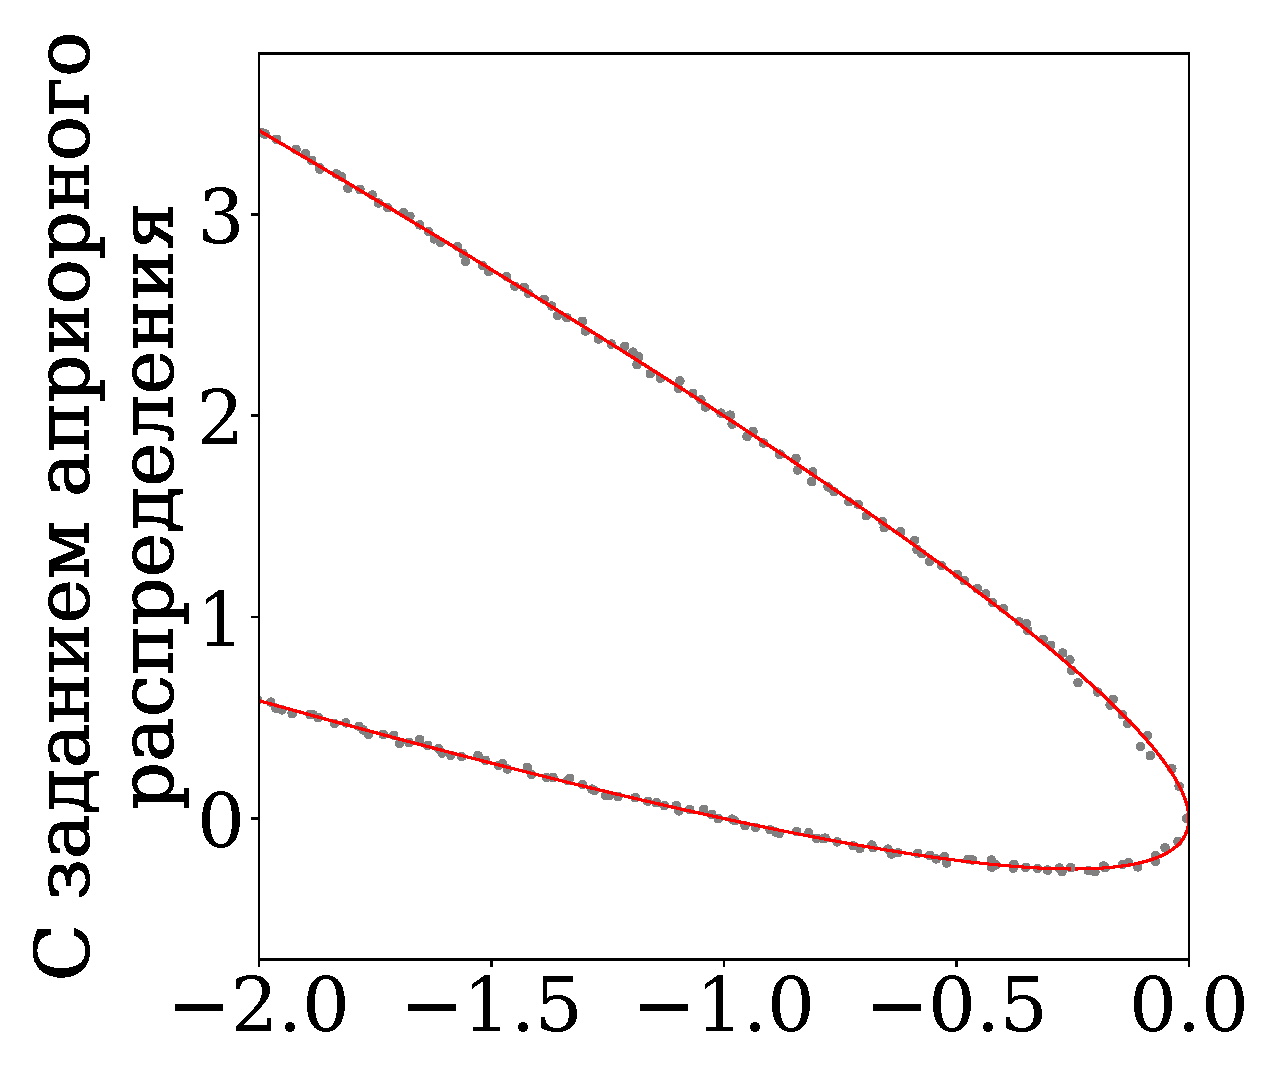
\includegraphics[scale = 0.4]{510.eps}
\end{minipage}
\begin{minipage}{.49\textwidth}
  \centering
  \vspace{1mm}
    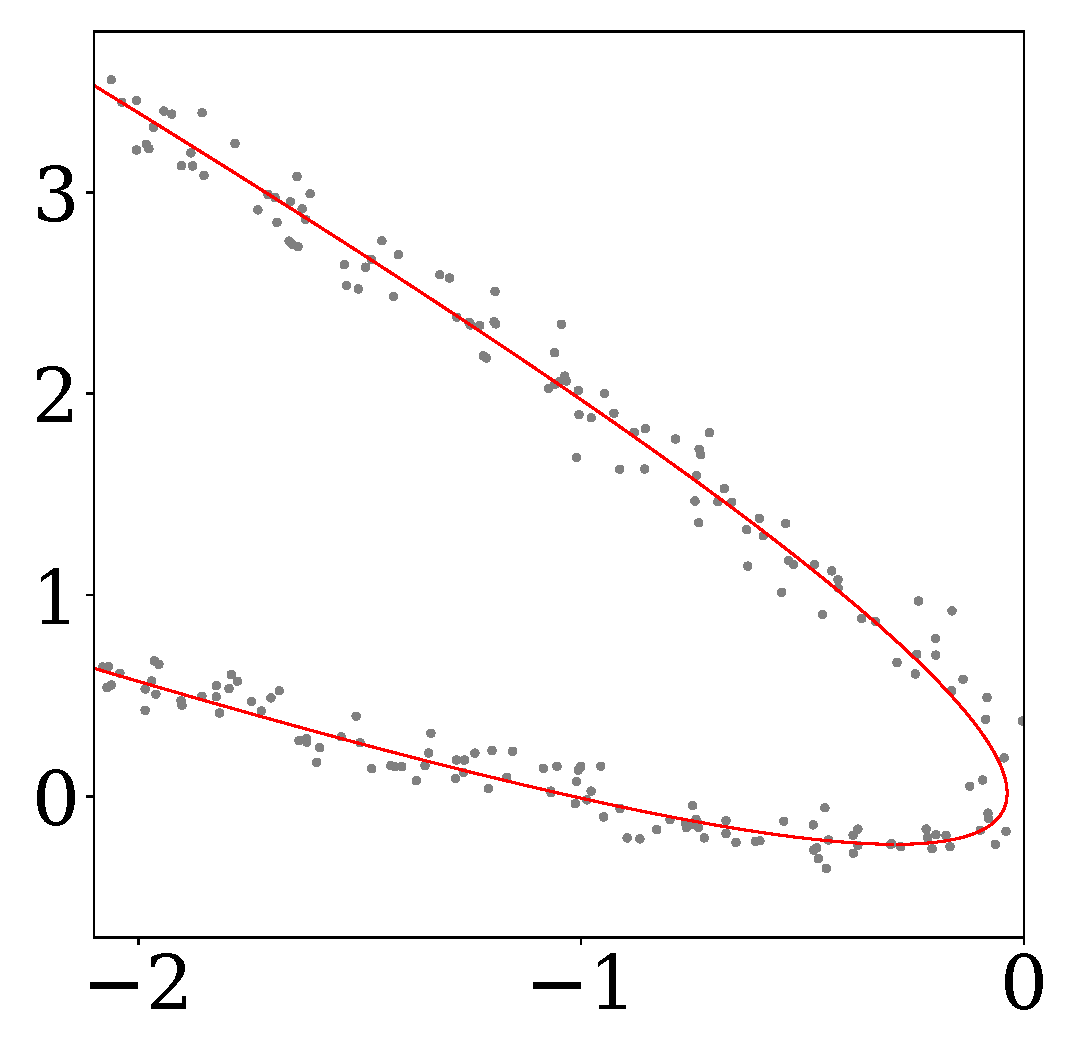
\includegraphics[scale = 0.4]{511.eps}
\end{minipage} 
\smallskip
\begin{minipage}{.49\textwidth}
 \centering
      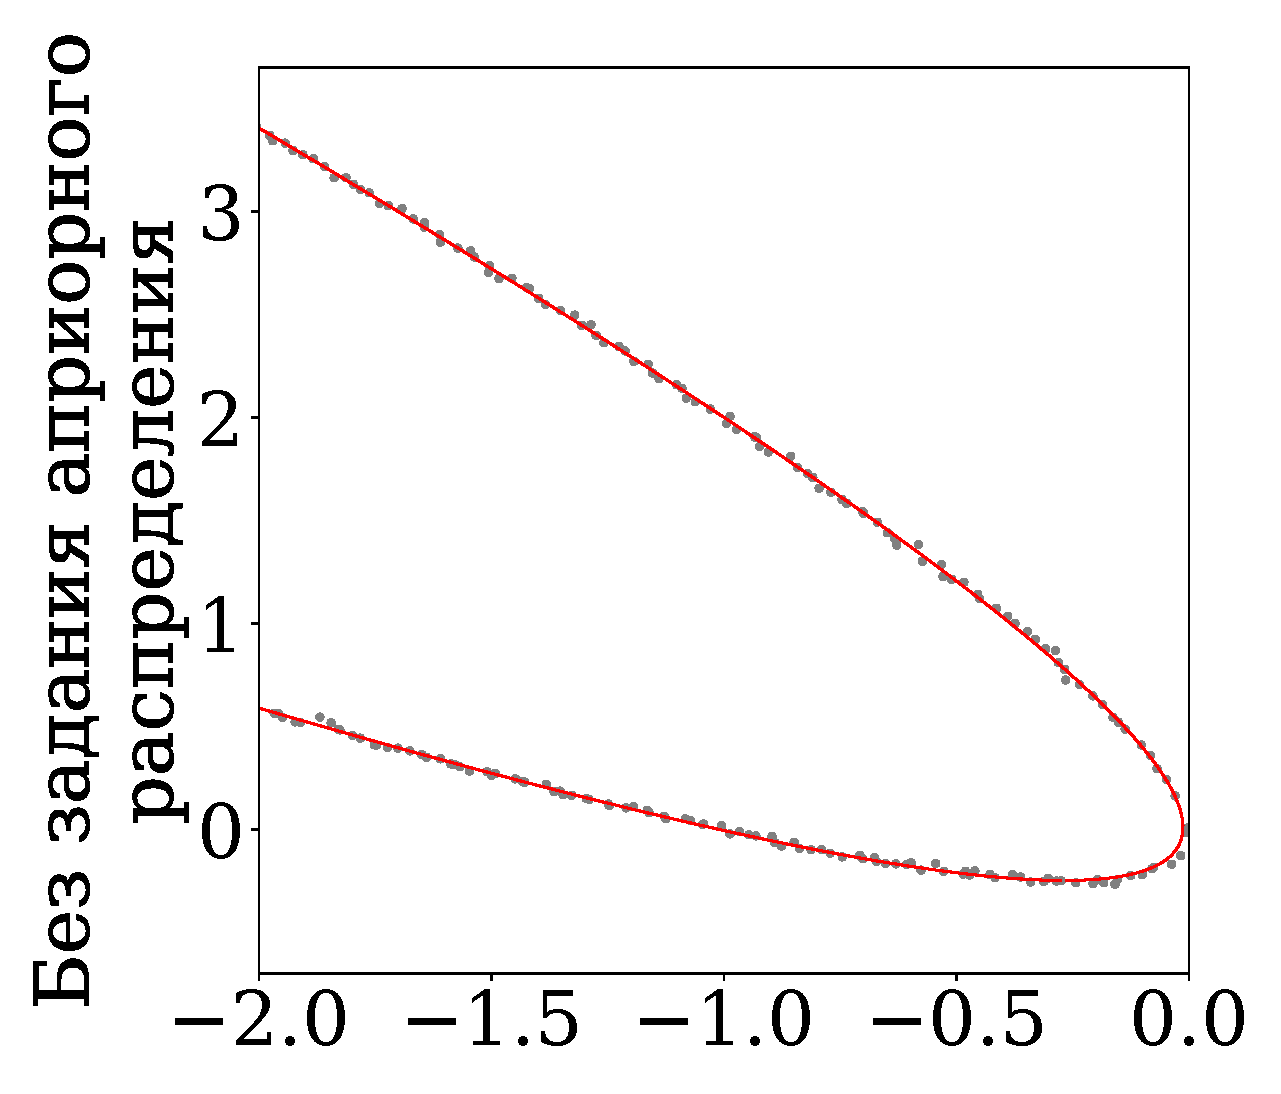
\includegraphics[scale = 0.4]{500.eps} 
    %\captionof{figure}{Эллипс}
\end{minipage}
\begin{minipage}{.49\textwidth}
  \centering
  \vspace{2mm}
  \hspace{4mm}
  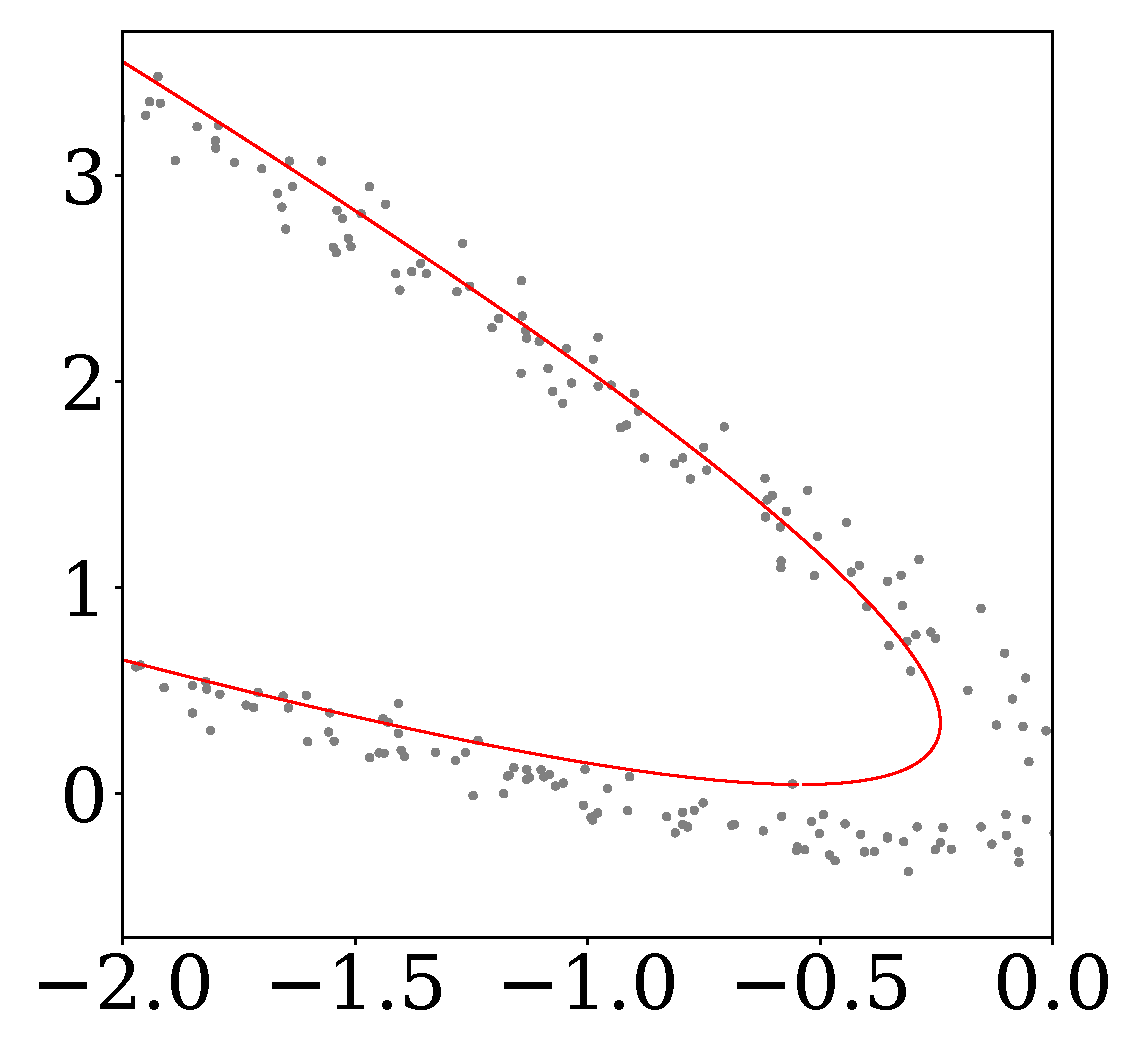
\includegraphics[scale = 0.4]{501.eps}
  %\captionof{figure}{Гипербола}
\end{minipage} 
\caption{Мультимодель в зависимости от разных априорных предположений и уровня шума.}
\end{figure}
Качество прогноза, вычисленное по формуле \ref{Sfunc}, в таблице 1:
\begin{table}[h!]
\centering
\begin{tabular}{|l|l|l|}
\hline
                     & $S_{\mathfrak{M}_1}$   & $S_{\mathfrak{M}_2}$  \\ \hline
$\text{Synthetic} 1$ & $10^{-5}$  & $10^{-4}$ \\ \hline
$\text{Synthetic} 2$ & $10^{-3}$ & $0.13$ \\ \hline
\end{tabular}
\end{table}

\begin{figure}
\begin{minipage}{.25\textwidth}
      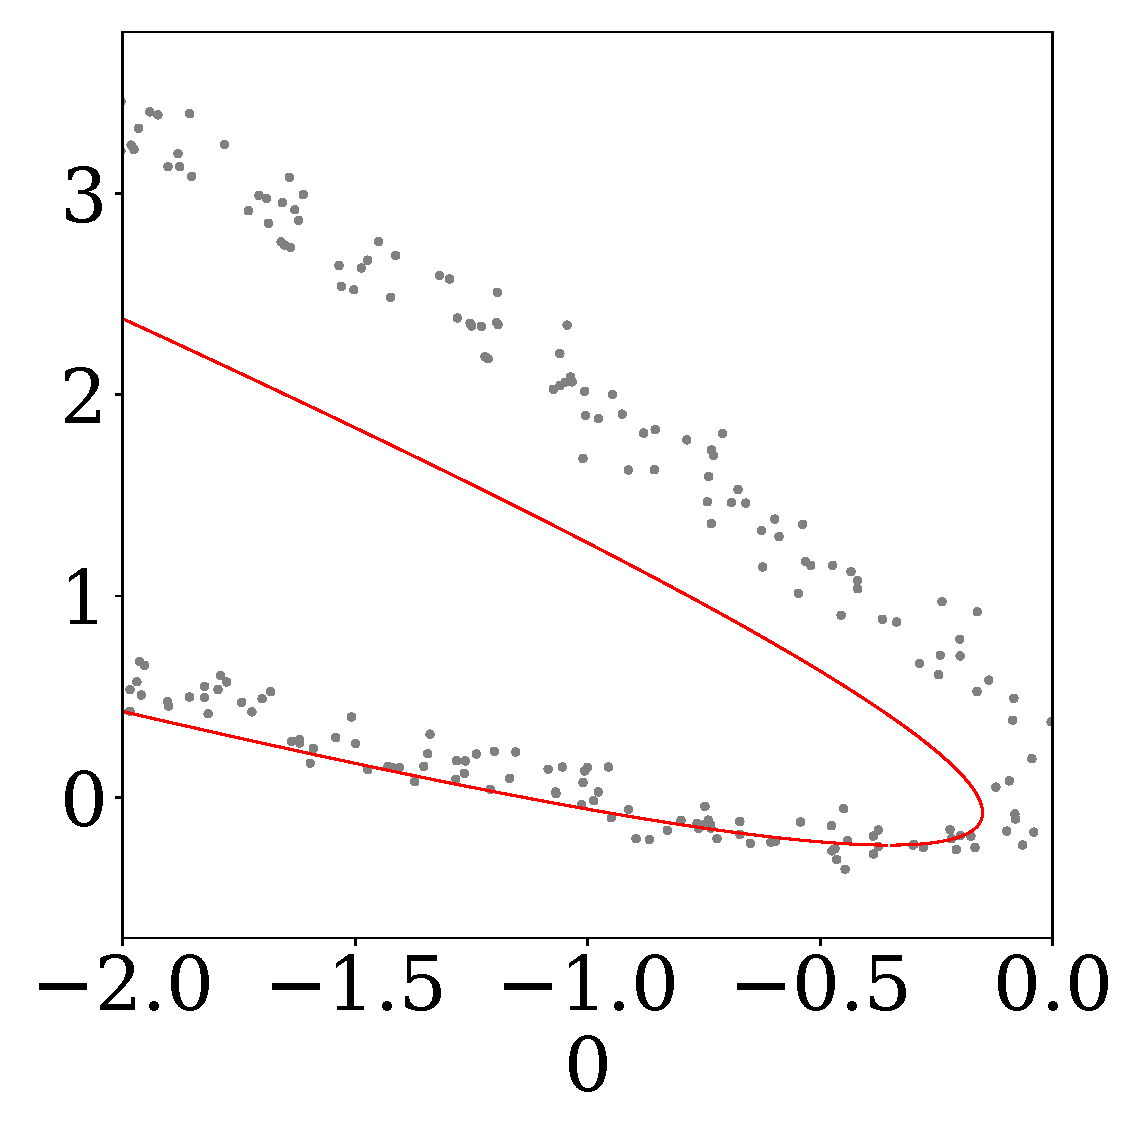
\includegraphics[scale = 0.19]{511_0.eps}
\end{minipage}
\begin{minipage}{.25\textwidth}

      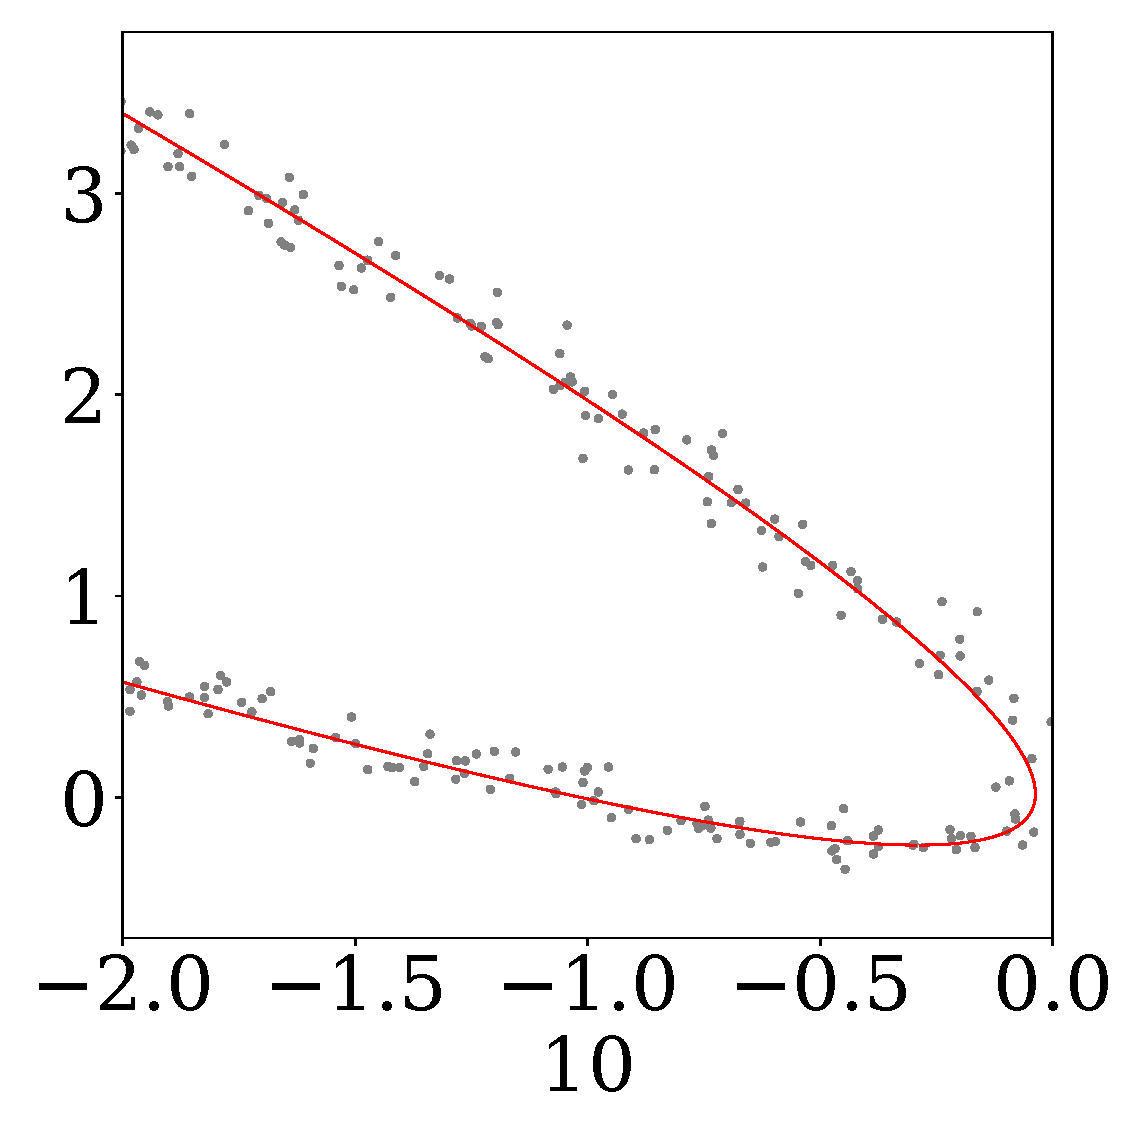
\includegraphics[scale = 0.19]{511_10.eps}
\end{minipage}
\begin{minipage}{.25\textwidth}

      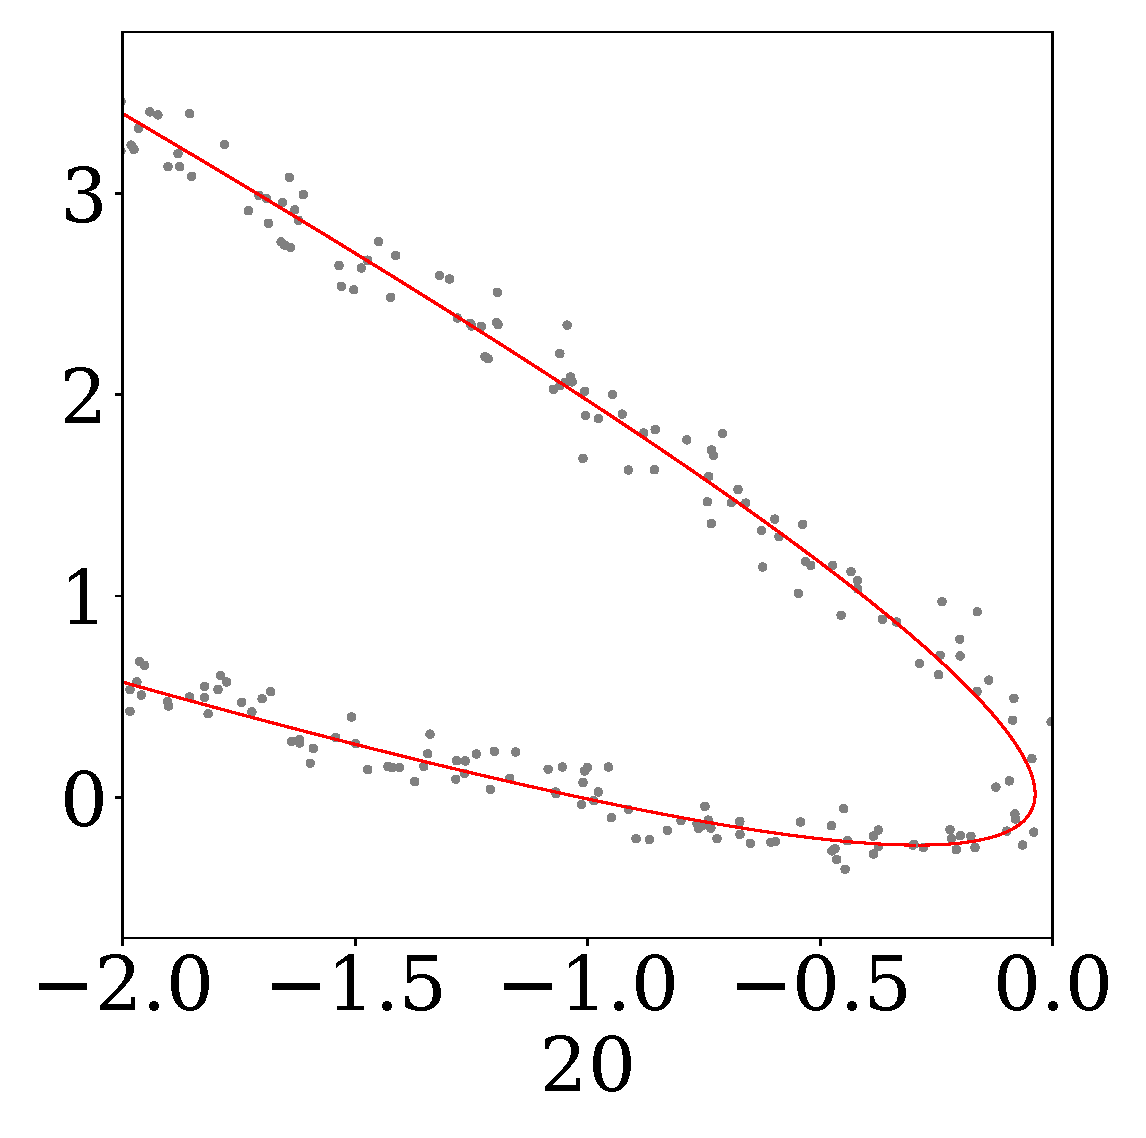
\includegraphics[scale = 0.19]{511_20.eps}
\end{minipage}
\begin{minipage}{.20\textwidth}

      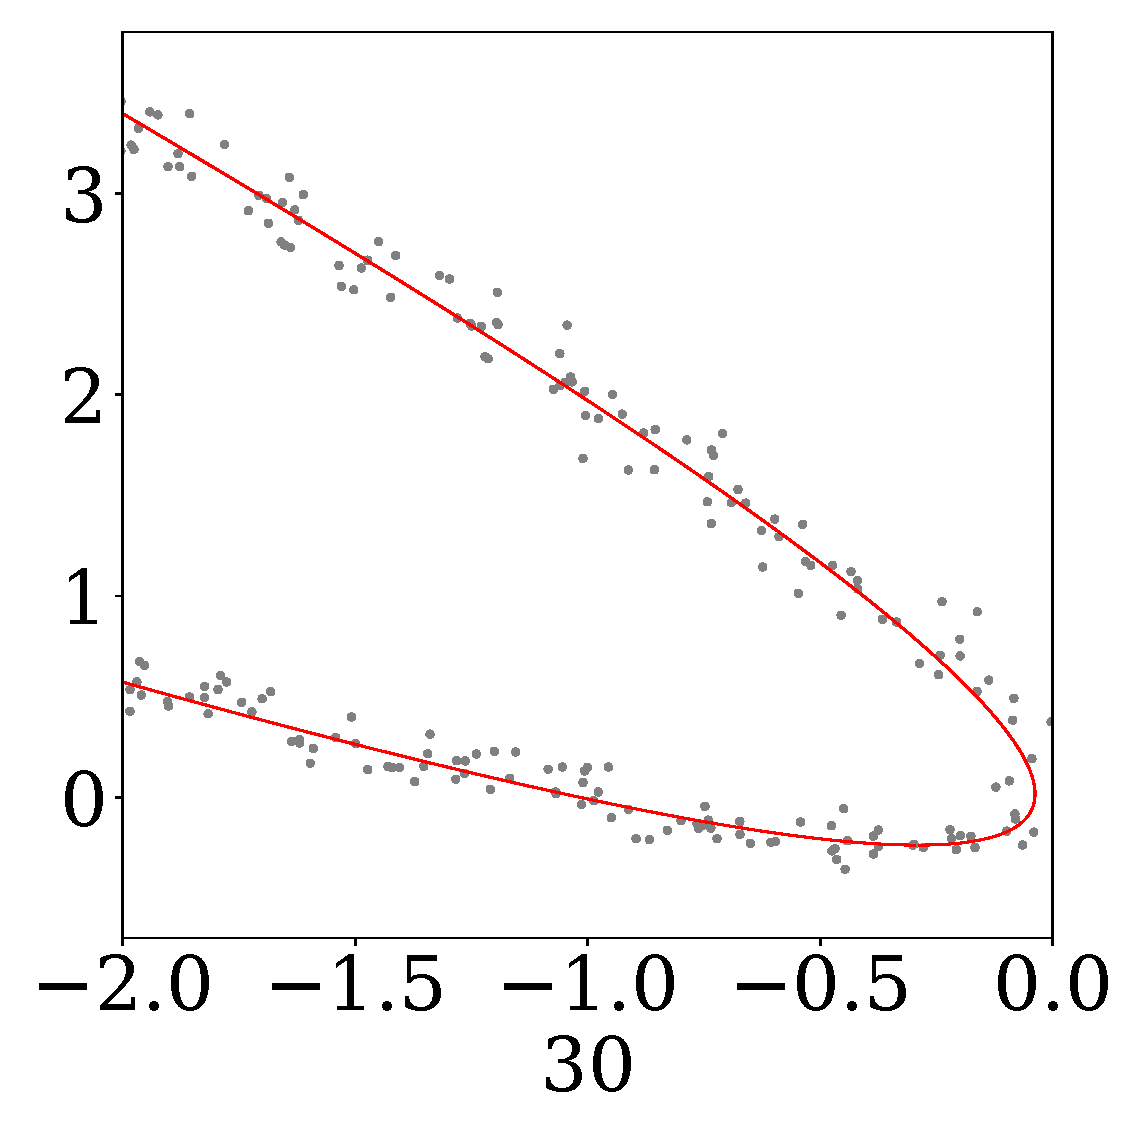
\includegraphics[scale = 0.19]{511_30.eps}
\end{minipage}
\caption{Визуализация процесса обучения мультимодели в течение 30 итераций}
\end{figure}
\begin{figure}[h!]
    \centering
    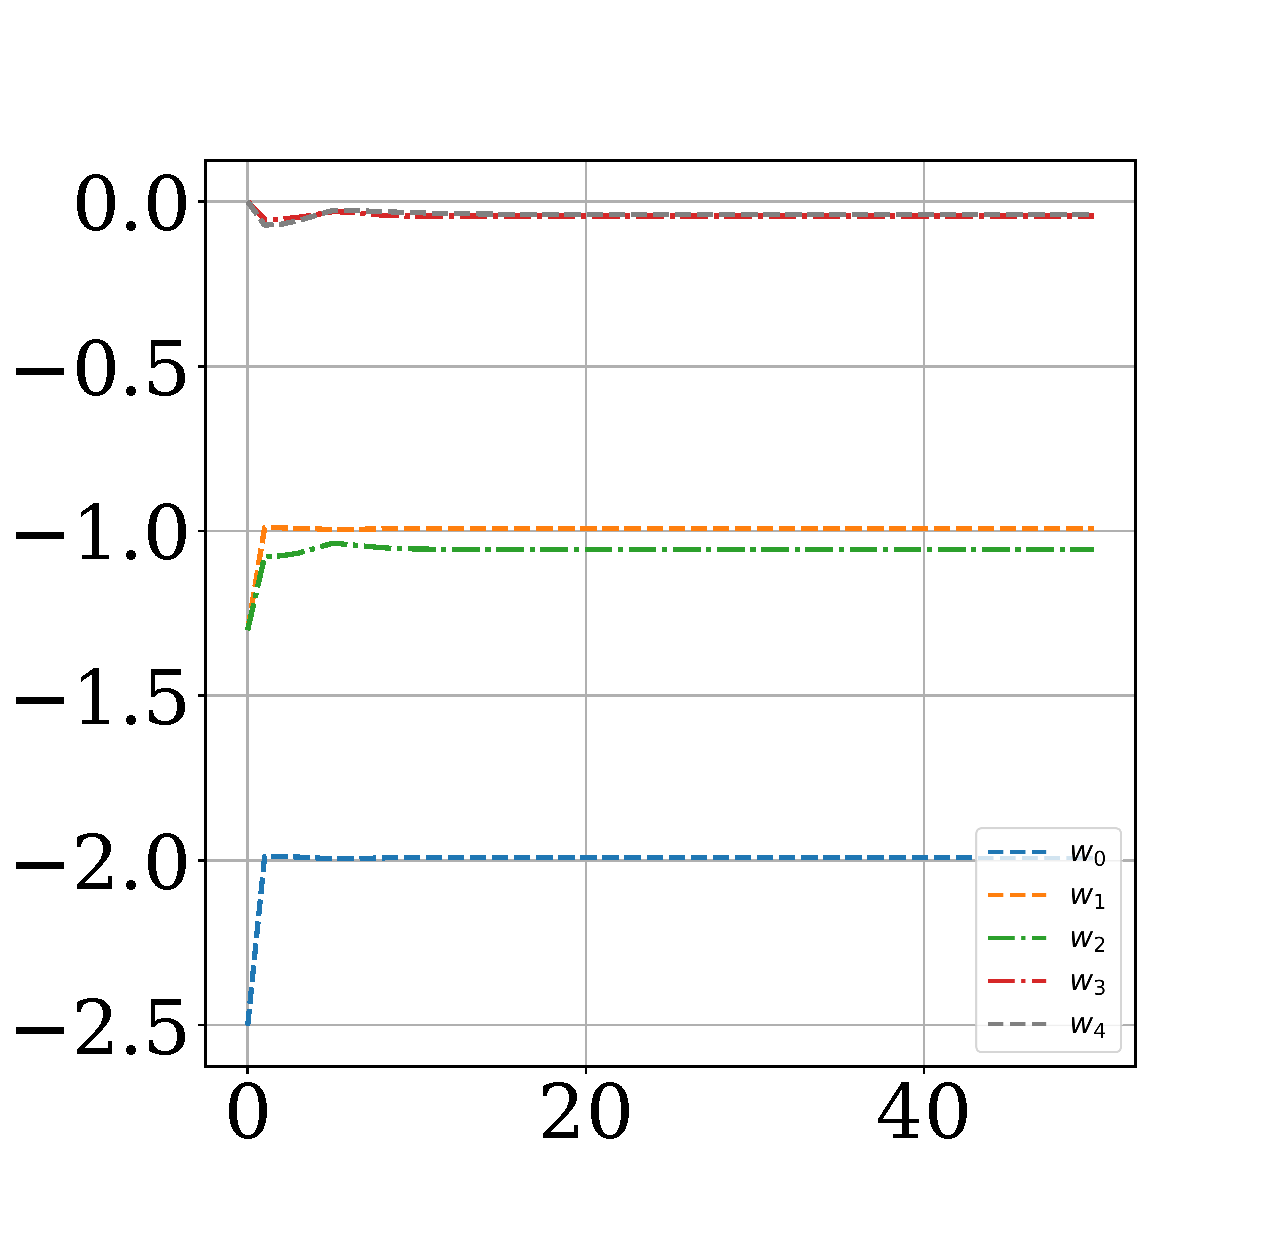
\includegraphics[scale = 0.5]{511w.eps}
    \caption{График зависимости $w_i$ от номера итерации}
\end{figure} 
На рис.~2 показан процесс обучения мультимодели $\mathfrak{M}_1$ на выборке Synthetic 2 в течение 30 итераций. \\
На рис.~3 изображены графики зависимости коэффициентов $w_i$ от номера итерации при работе модели $\mathfrak{M}_2$ на выборке Synthetic 2.\\
В ходе эксперимента показано, что задание априорного распределения улучшает качество распознавания изображений.\\
\textbf{Анализ мультимодели в зависимости от шума.}  Для анализа свойств мультимоделей $\mathfrak{M}_1$ и $\mathfrak{M}_2$ в зависимости от зашумленности изображения проведен вычислительный эксперимент на выборках Synthetic 3, Synthetic 4 и Synthetic 5. Минимальный уровень шума равен 0, когда на изображении нет шумовых точек, а максимальный равен $0.15$, когда на изображении число шумовых точек равно $\frac{1}{6}$ от числа точек всех окружностей. Работа мультимодели на данных выборках с заданным априорным распределением и без задания априорного распределения показана на рис. 4.\\
На рис. 5 показан график зависимости радиуса $r$ и центра $(x_0, y_0)$ от номера итерации для каждой окружности. Нетрудно видеть, что  модель $\mathfrak{M}_1$ с заданием априорного распределения сходится быстрее, чем модель $\mathfrak{M}_2$ без задания, и является более устойчивой к шуму. Качество работы обеих моделей снижается при работе на равномерно зашумленных данных. При этом $\mathfrak{M}_1$ разделяет точки исходных окружностей точнее, чем $\mathfrak{M}_2$, однако из-за наличия шумовых точек параметры окружностей, найденные $\mathfrak{M}_1$, не совпадают с истинными параметрами.
\begin{figure}[h!]
\begin{minipage}{.32\textwidth}
      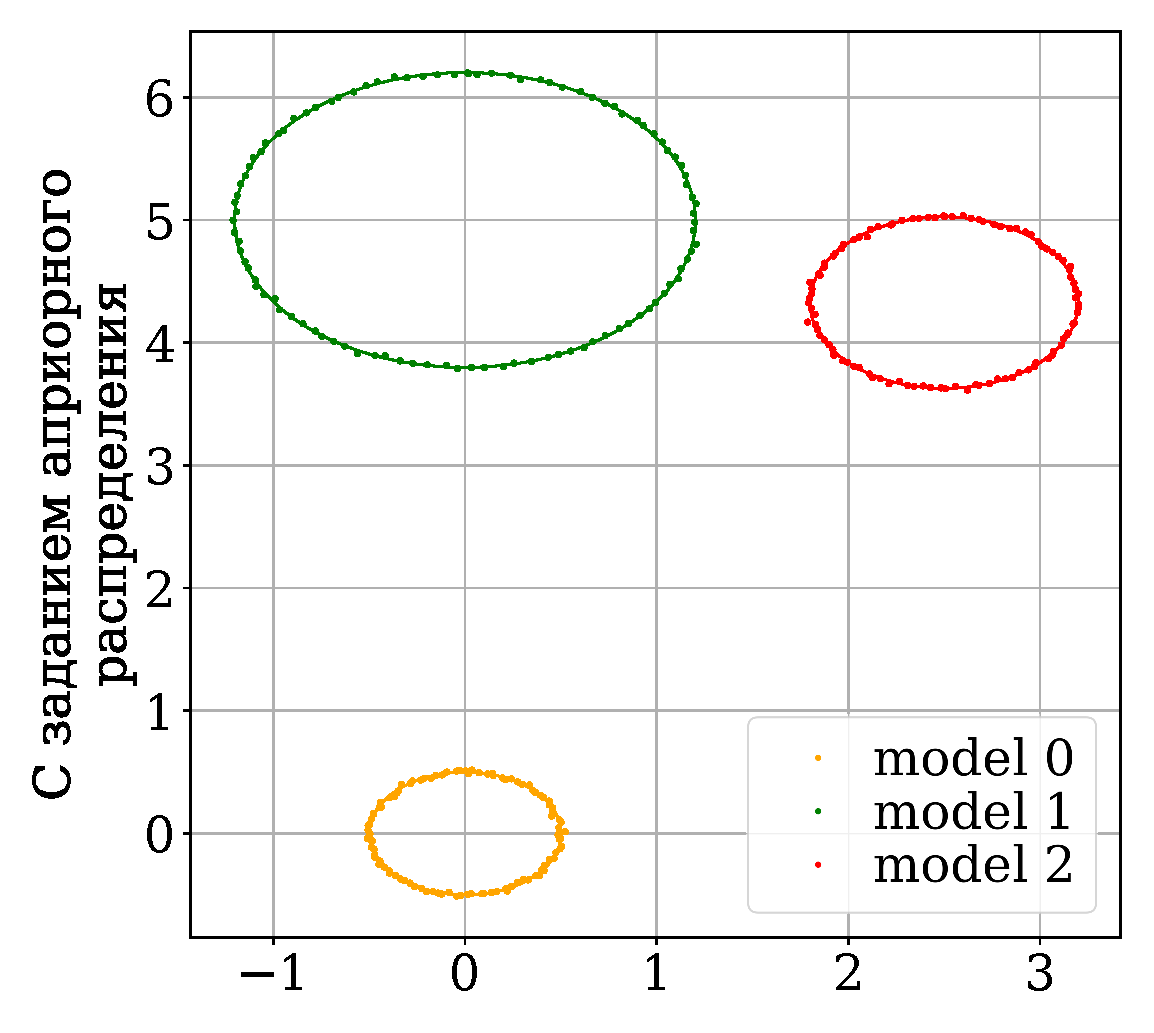
\includegraphics[width =  \textwidth]{910.eps}
\end{minipage}
\begin{minipage}{.32\textwidth}
\hspace{0.3mm}
      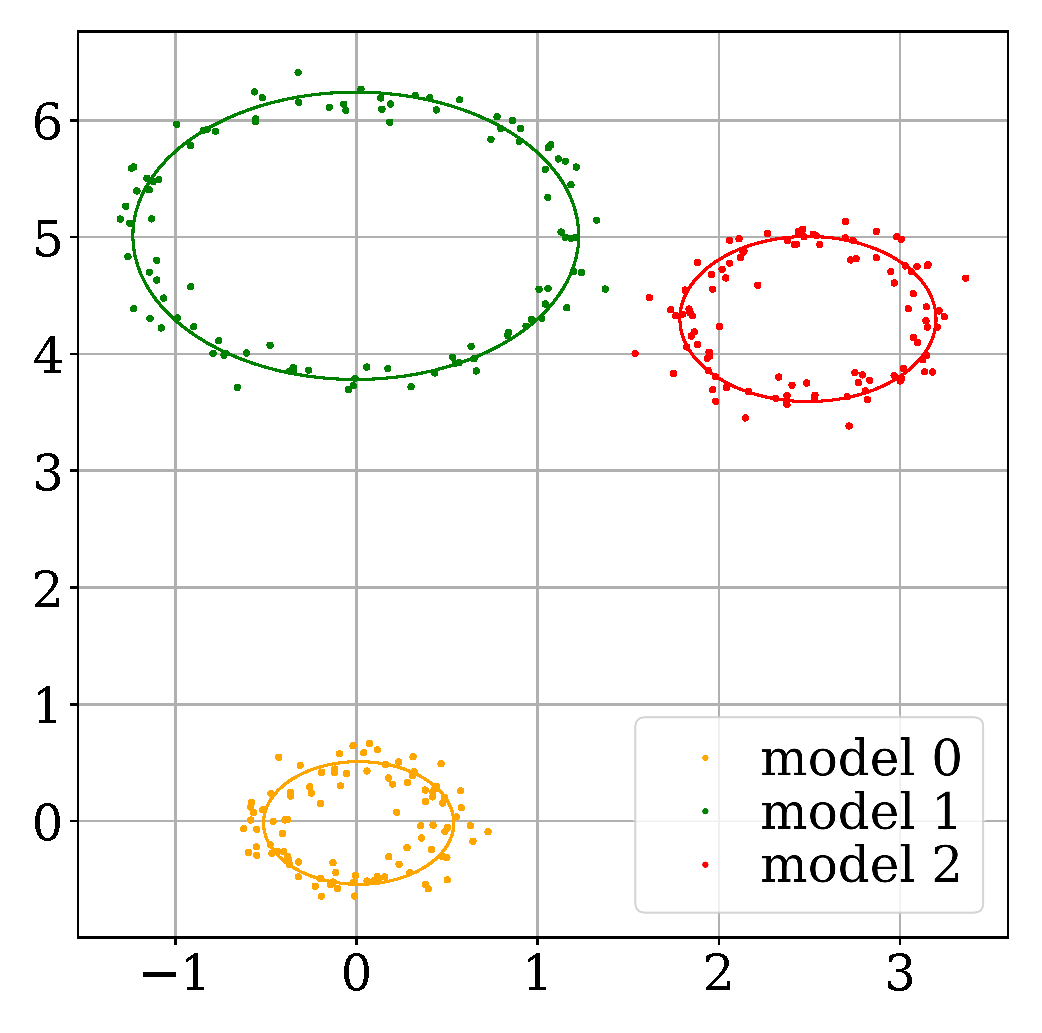
\includegraphics[width =  0.89\textwidth]{901.eps}
\end{minipage}
\begin{minipage}{.32\textwidth}
\vspace{-3mm}
\hspace{-8.5mm}
      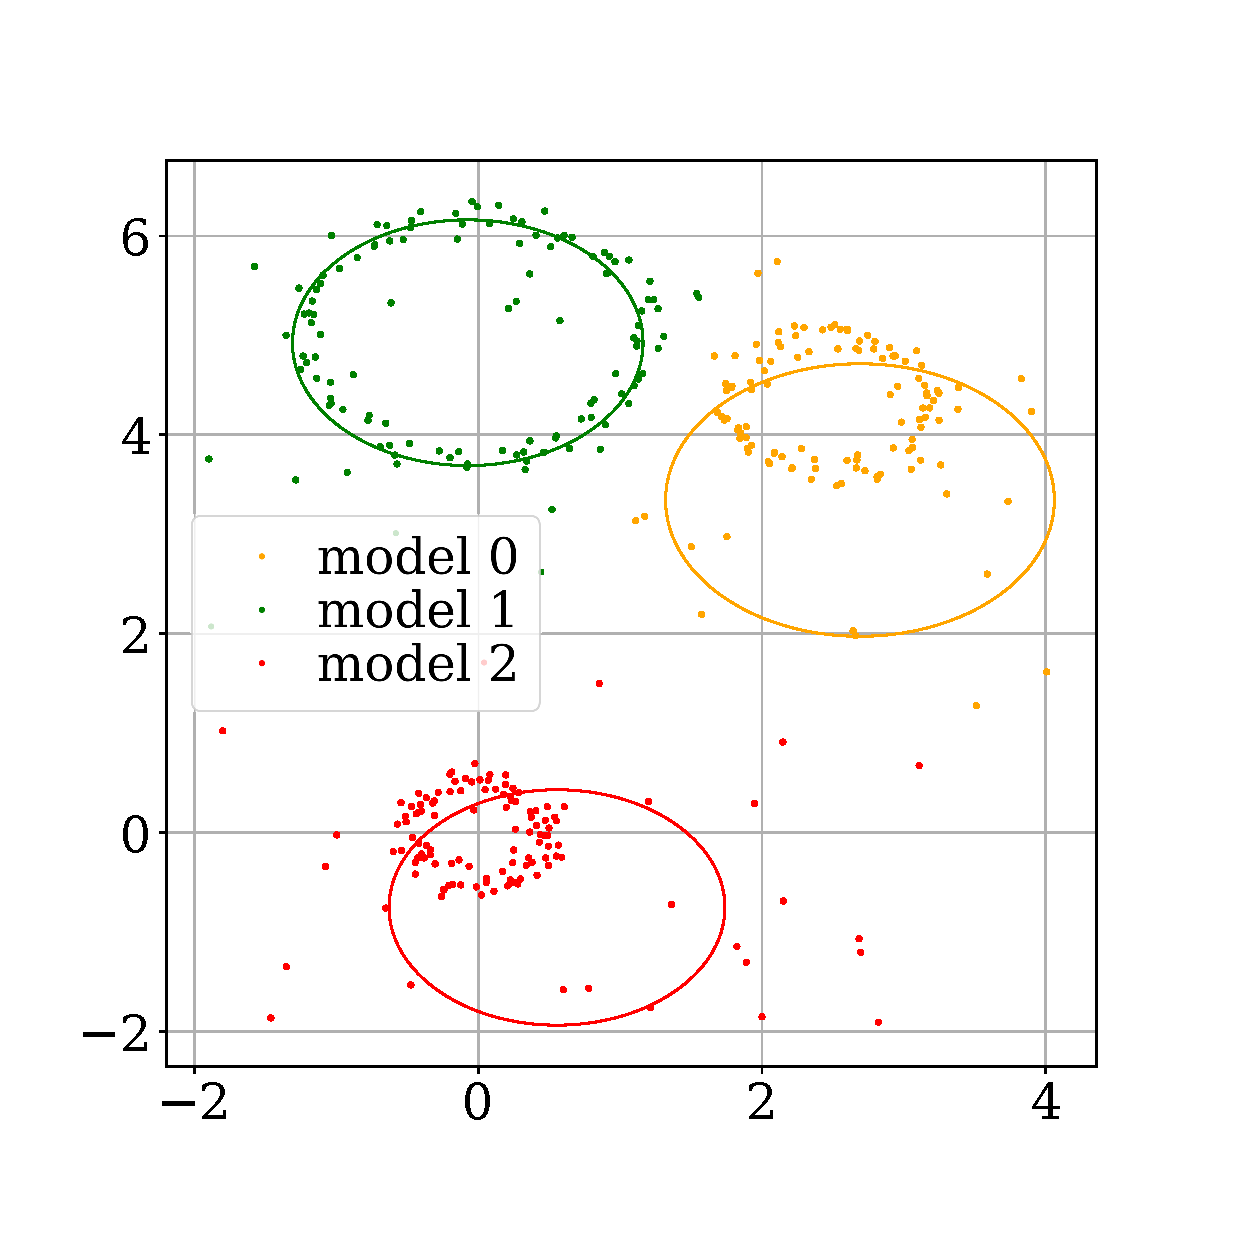
\includegraphics[width =  1.07\textwidth]{902.eps}
\end{minipage}
\begin{minipage}{.32\textwidth}
      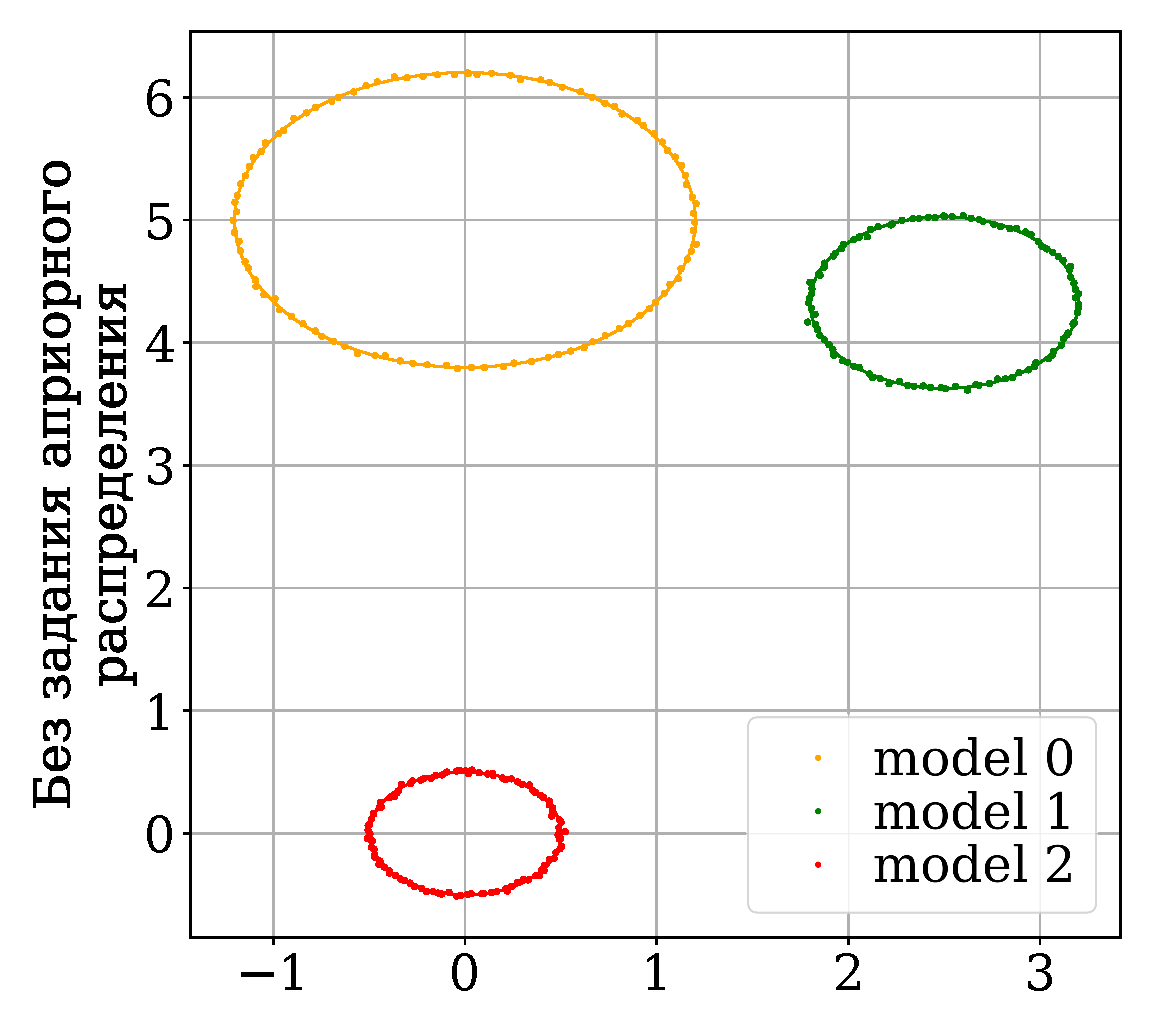
\includegraphics[width =  \textwidth]{900.eps}
\end{minipage}
\begin{minipage}{.32\textwidth}
\hspace{2mm}
      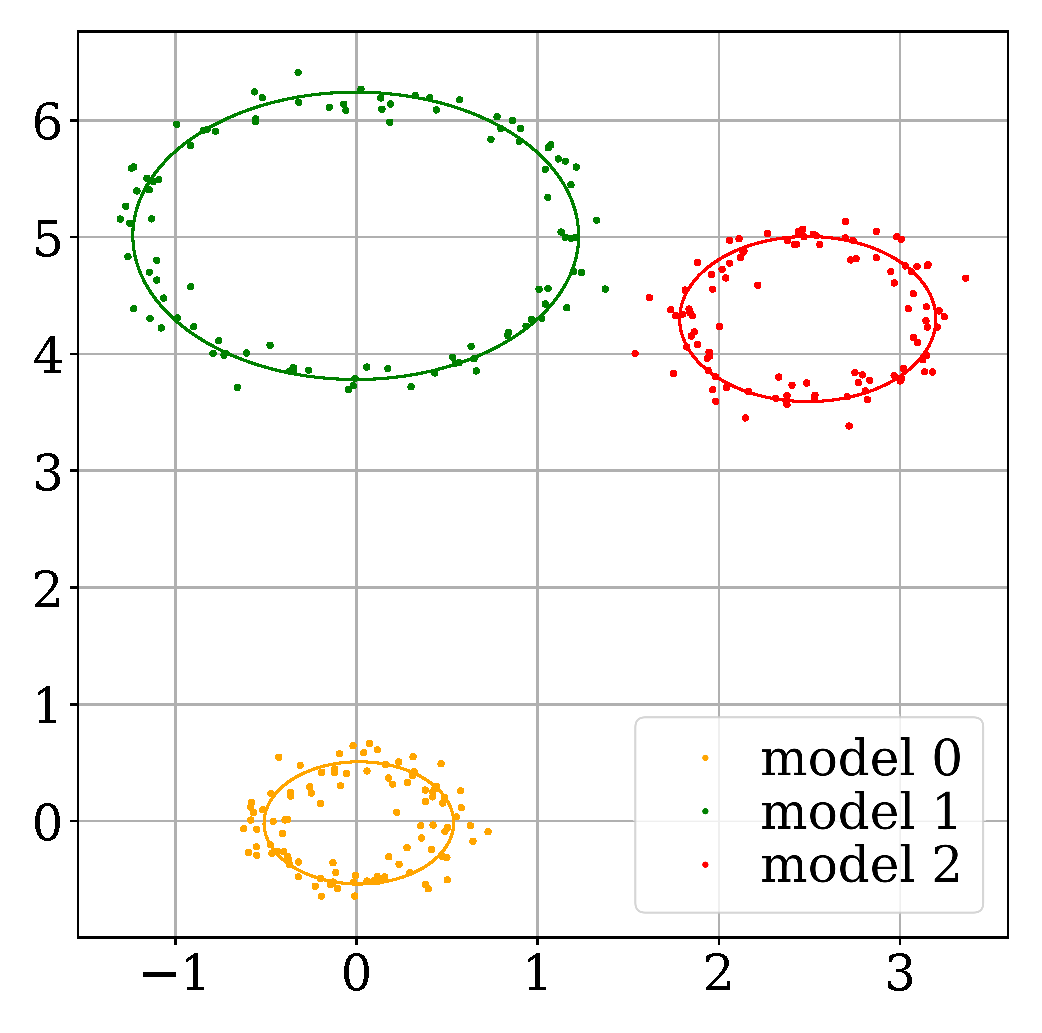
\includegraphics[width =  0.9\textwidth]{911.eps}
\end{minipage}
\begin{minipage}{.32\textwidth}
\hspace{-2.3mm}
      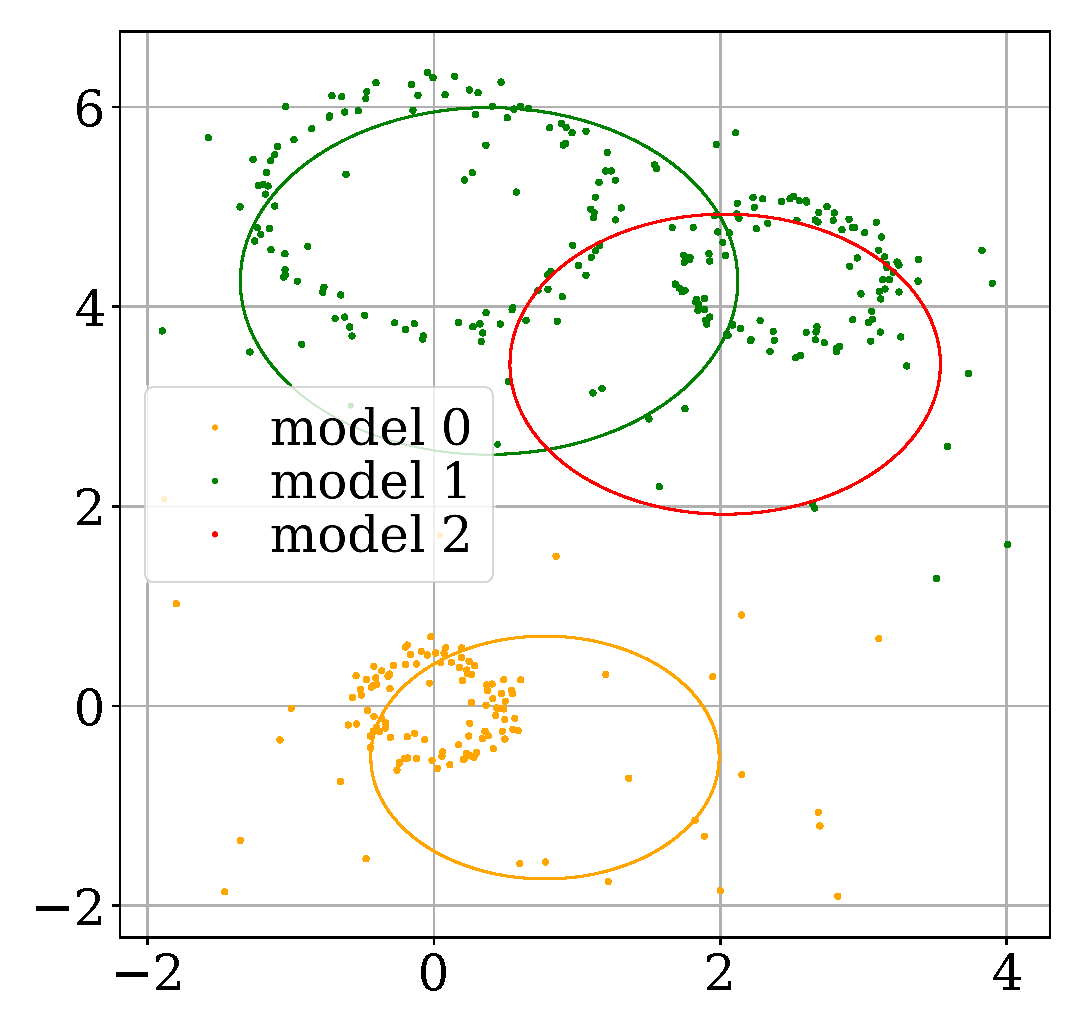
\includegraphics[width =  0.935\textwidth]{912.eps}
\end{minipage}
\caption{Мультимодель в зависимости от разных априорных предположений и уровня шума}
\end{figure}

\begin{figure}[h]
\begin{minipage}{.32\textwidth}
\hspace{-3mm}
      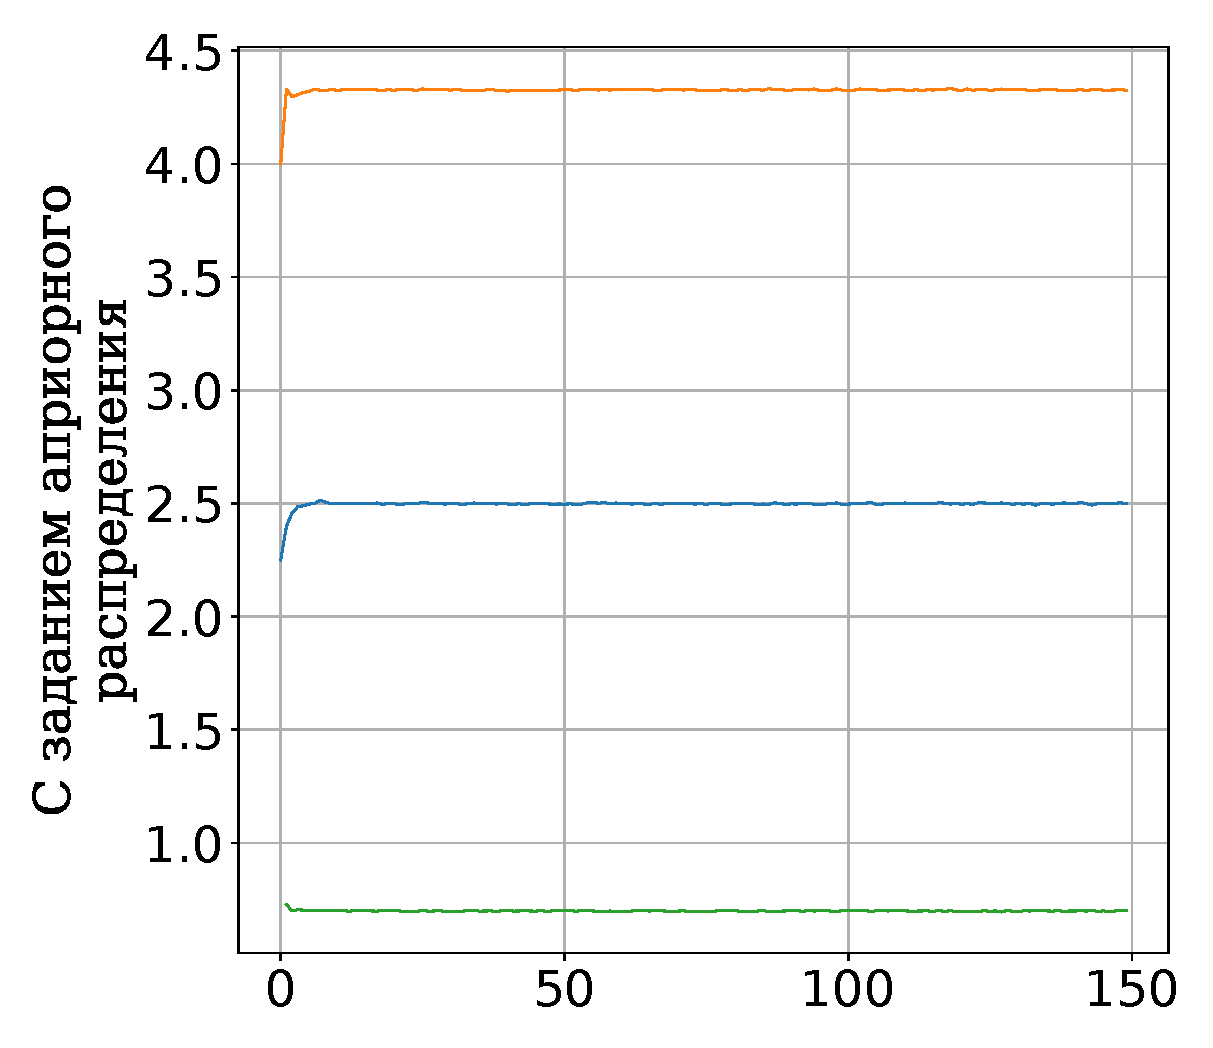
\includegraphics[width = 1.05\textwidth]{910noise.eps}
\end{minipage}
\begin{minipage}{.32\textwidth}
\vspace{2pt}
\hspace{-2.1mm}
      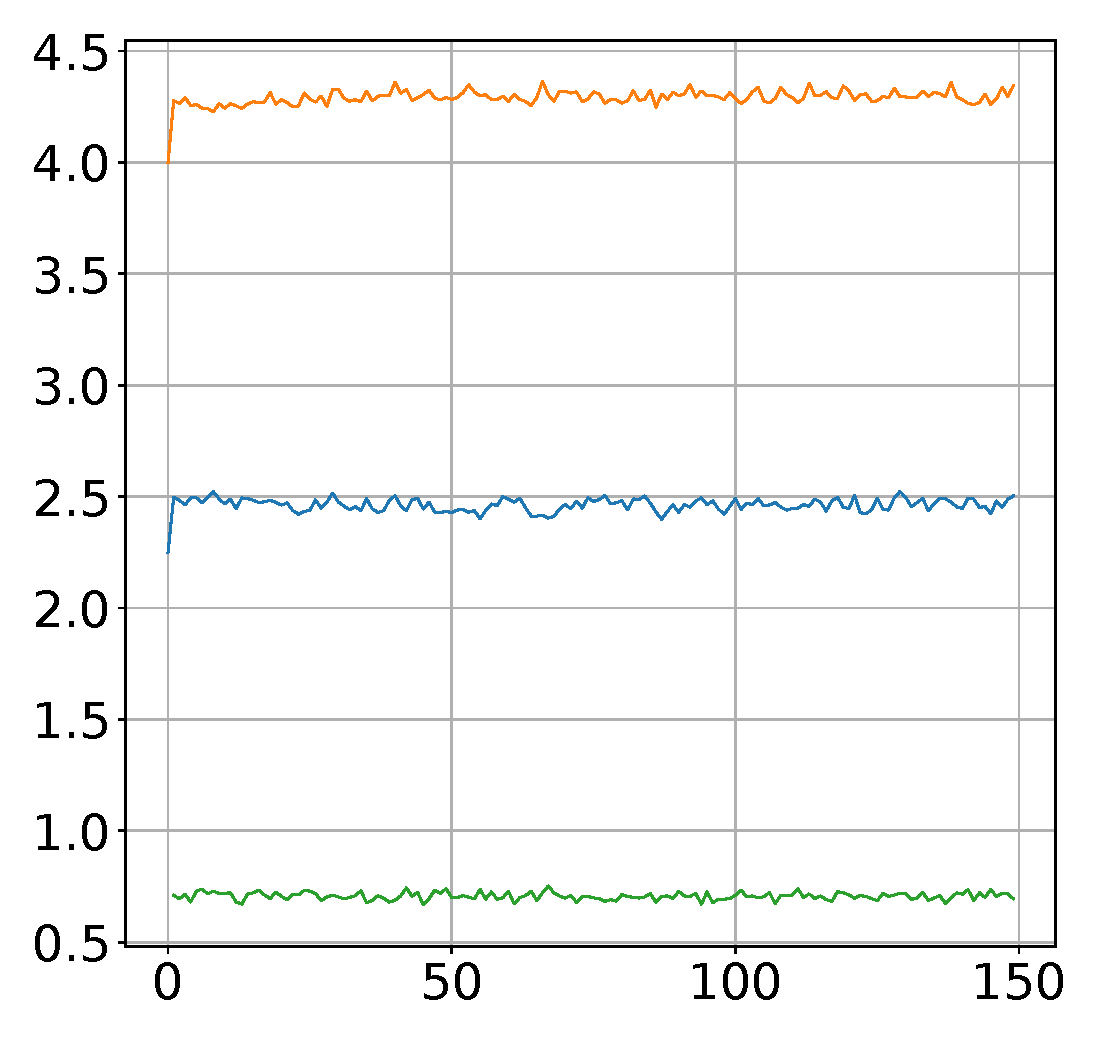
\includegraphics[width = 0.95\textwidth]{911noise.eps}
\end{minipage}
\begin{minipage}{.32\textwidth}
\vspace{2pt}
\hspace{-6.3mm}
      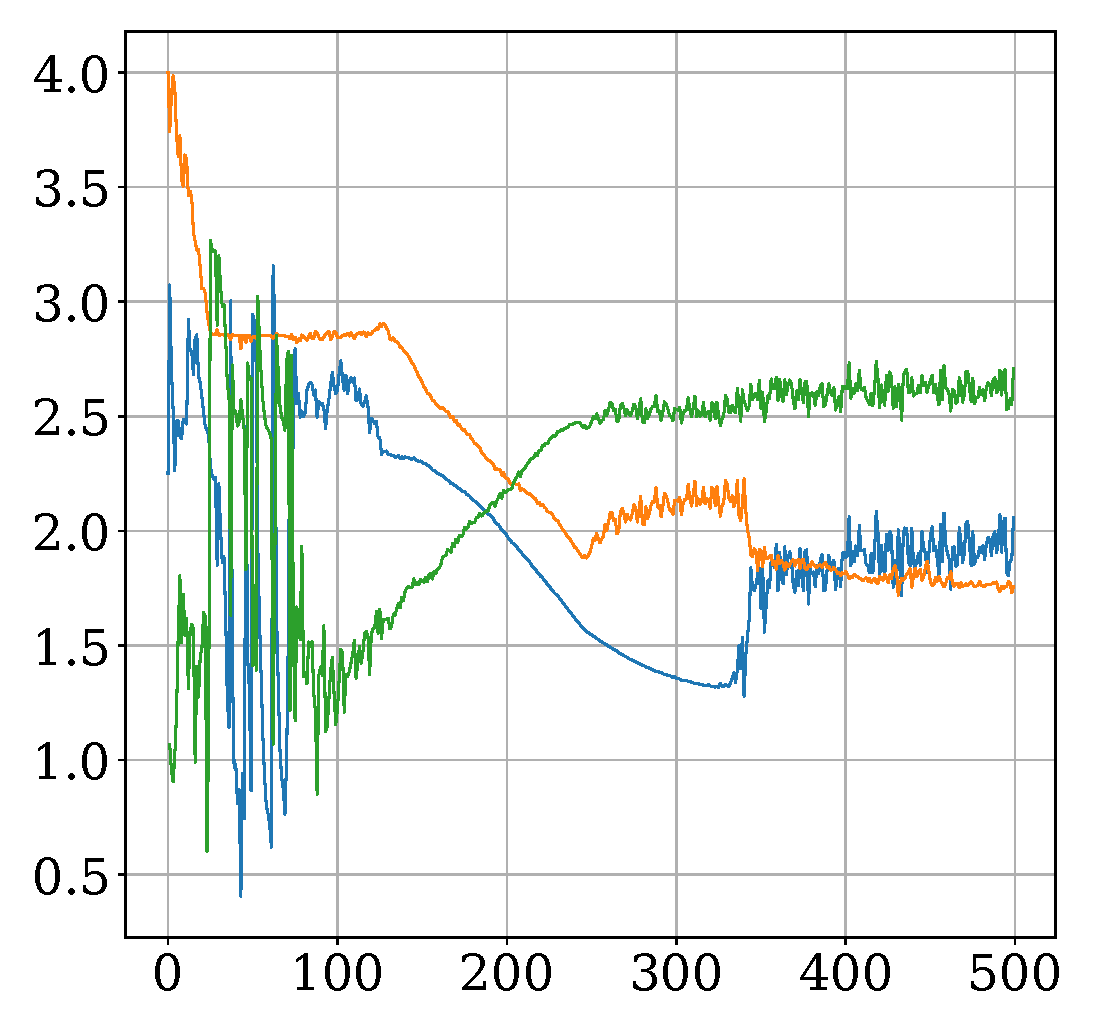
\includegraphics[width = 0.95\textwidth]{912noise.eps}
\end{minipage}
\begin{minipage}{.32\textwidth}
\hspace{-3mm}
      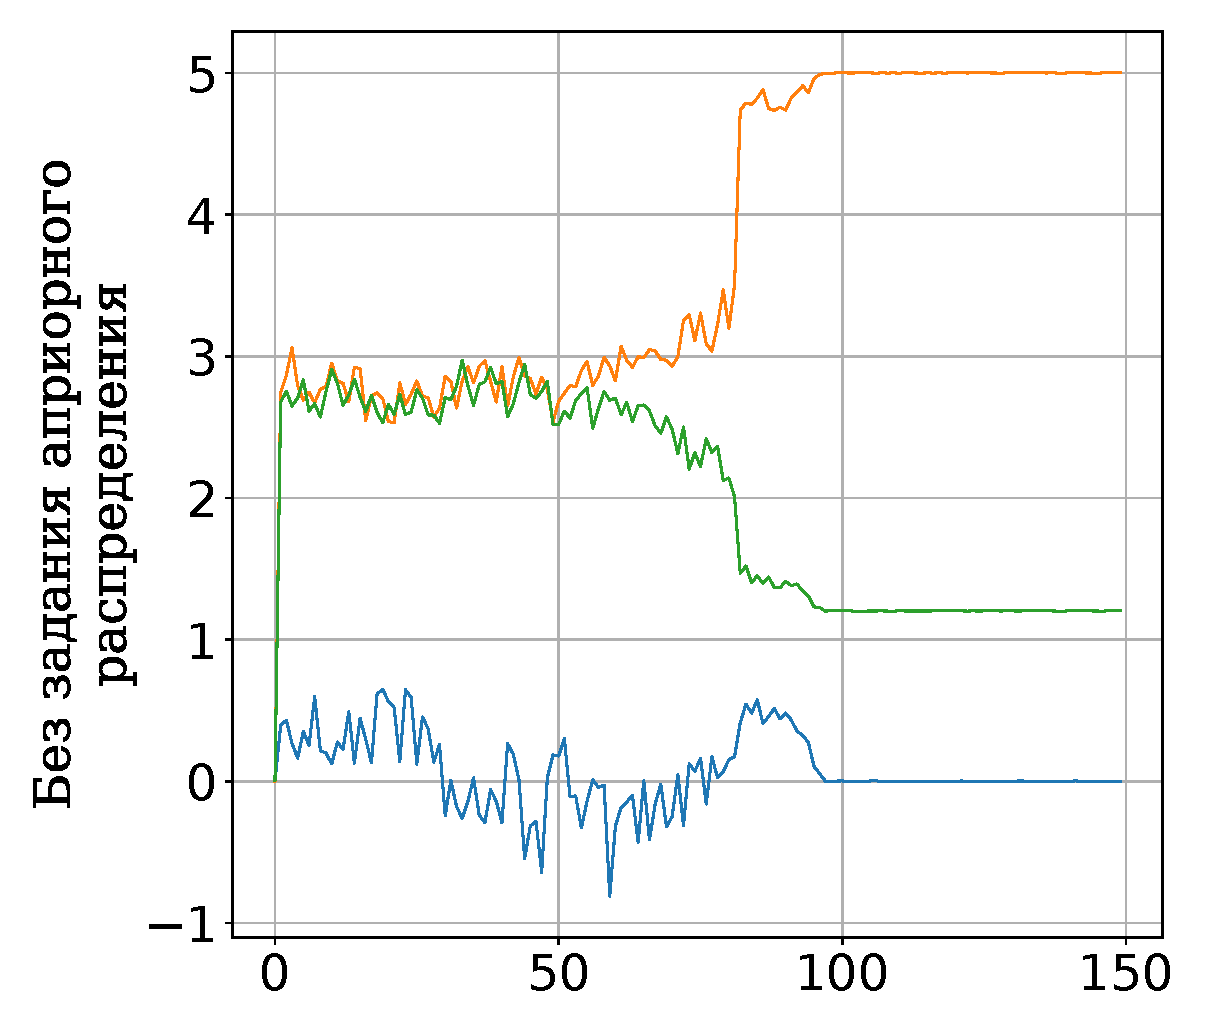
\includegraphics[width = 1.05\textwidth]{900noise.eps}
\end{minipage}
\begin{minipage}{.32\textwidth}
\hspace{-2.1mm}
      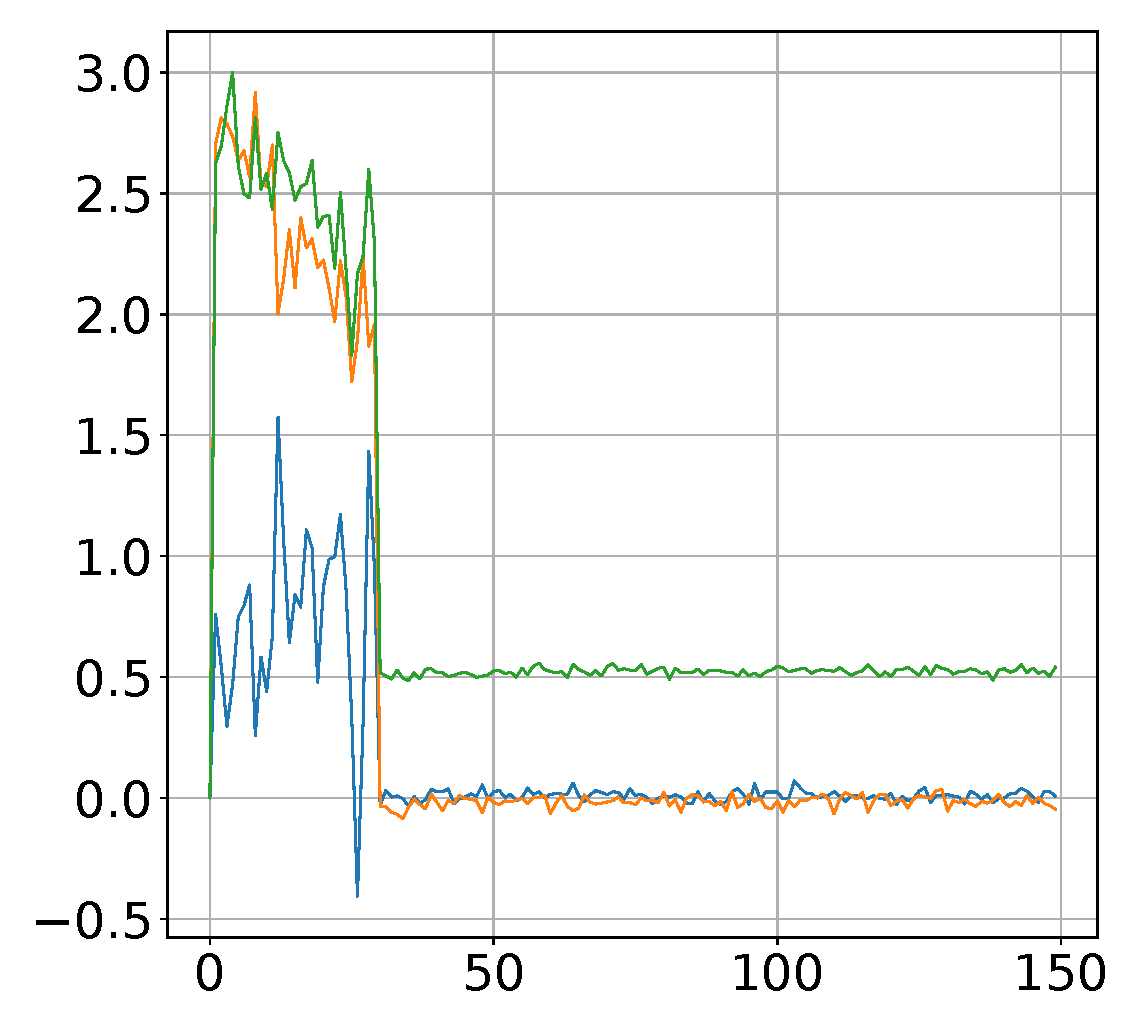
\includegraphics[width = \textwidth]{901noise.eps}
\end{minipage}
\begin{minipage}{.32\textwidth}
\hspace{-2mm}
      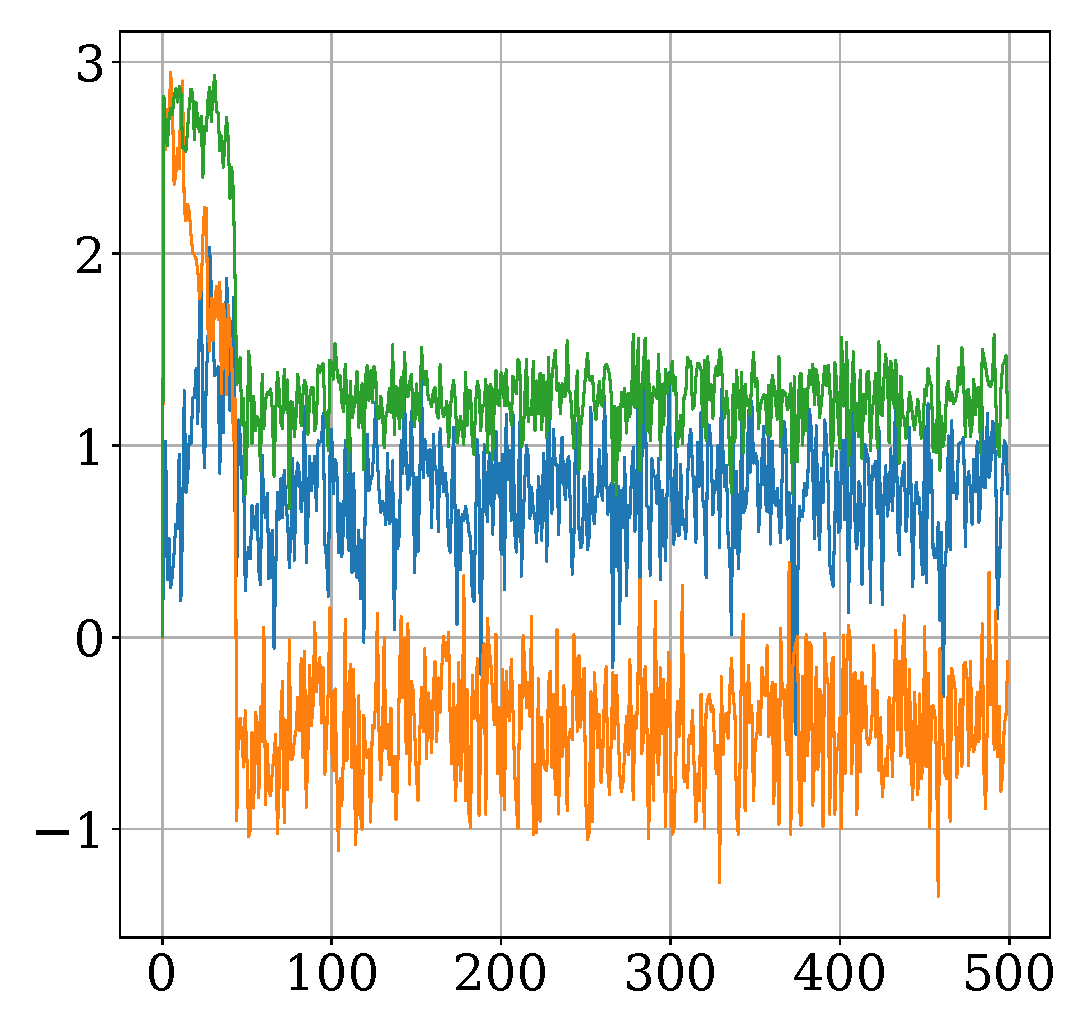
\includegraphics[width = 0.95\textwidth]{902noise.eps}
\end{minipage}
%\begin{center}
\caption{Зависимость параметров $r$, $x_0$ и $y_0$ от номера итерации при разных априорных распределениях}
\end{figure}
%\textbf{Рис. 5} Зависимость параметров $r$, $x_0$ и $y_0$ от номера итерации при разных априорных распределениях
%\end{center} 
\vspace{30mm}
%далее сам список используевой литературы
Данный эксперимент демонстрирует, что модель $\mathfrak{M}_1$ с заданием априорного распределения более устойчива к шуму. $\mathfrak{U}$
\newpage
\section{Список литературы}
\hspace{-6 mm}$[1]$ \textit{Graboviy\,A.\,V., Strijov\,V.\,V.} Analysis of prior distributions for a mixture of experts // Computational Mathematics and Mathematical Physics, to appear in 2020. \\
$[2]$ \textit{Scheres\,S.\,H.\,W.} A Bayesian view on Cryo-EM structure determination. // Journal of Molecular Biology. 2012. Vol.\,415. \No\,2. P. 406--418.\\
$[3]$ \textit{Yuksel\,S.\,E., Wilson\,J.\,N., Gader\,P.\,D.} Twenty years of mixture of experts // IEEE Transactions on Neural Networks and Learning Systems. 2012. Vol.\,23, \No\,8, P. 1177--1193.
$[4]$ \textit{Matveev\,I.\,A.} Detection of iris in image by interrelated maxima of brightness gradient projections //  Applied and Computational Mathematics. 2010. Vol.\,9. \No\,2. P. 252--257. \\
\end{document}